\chapter{The Large Hadron Collider and the CMS Detector}

The searches for new physics discussed in the next chapter analyze data recorded by the Compact Muon Solenoid (CMS) experiment.
The CMS detector itself straddles beams generated by the Large Hadron Collider (LHC), a particle collider located at CERN in Geneva, Switzerland.
CMS directly measures the products of collisions between the protons in these beams, digitizes the measurements, and records a small subset of these events.
The data is then processed by reconstruction algorithms and shared across the worldwide CMS computing grid.
This chapter describes the LHC and CMS.

\section{The Large Hadron Collider} \label{sec:LHC}

A detailed description of the LHC is available in Reference~\cite{LHC_TDR}.
This section provides a summary of the essential information.

  \subsection{A Brief Description} \label{sec:LHCdescription}

  Although it sometimes collides atomic nuclei, typically Pb-208, the LHC is primarily a proton-proton collider, and that is the operational mode we shall consider in this work.
  The LHC is the highest energy and highest luminosity proton-proton collider ever constructed, thus far achieving collisions with center of momentum frame energy as large as 13\~TeV, produced by two counterrotating beams of 6.5\~TeV protons, at sustained rates on the order of one billion collisions per second.

  Producing such high energy collisions at such high intensity requires that the LHC be a large ring, 27~km in circumference.
  The circular shape allows multiple opportunities for the protons in each beam to collide, rather than a single all-or-nothing pass, and additionally allows the beams to be circulated for as long as necessary to accelerate them up to the intended energy, at a rate of 0.5~MeV per revolution.
  The size makes it possible for the protons to be constrained to travel in a circle, even at very high energies.
  The beams are constrained to travel in the ring using powerful magnetic fields, and the maximum feasible magnetic field strength is the primary limit on the maximum achievable beam energy.
  The LHC beams require an 8.36~T field to stay on track, provided by superconducting niobium-titanium electromagnets carrying a current of 11,080\~A.
  Superconductors stable at greater magnetic field strengths are rare and expensive, and the magnets must be superconducting to carry such enormous currents.
  Larger rings reduce the beams' curvature and allow for greater energies with the same magnetic field strength.

  Protons are chosen for the beams rather than electrons, the only other obvious potential choice, for two reasons.
  First, protons are composite particles, so their total energies are distributed among their many subcomponents, referred to as partons in this context.
  Collisions between protons with energy 6.5~TeV each are in fact collisions between a parton in each proton with some fraction of the total energy.
  This naturally scans across the accessible energy range, providing sensivity to any new state with mass on the TeV scale.
  Were the beams composed of elementary particles like electrons, the collider would need to scan the beam energy to provide sensitivity to any possible mass.
  Therefore, electron colliders are poorly suited for new discoveries compared to proton colliders, and better suited for studying a state with known mass in greater detail.
  Second, and more importantly, the mass of the proton is much greater than that of the electron, reducing energy losses to synchrotron radiation.
  Because synchrotron losses are relatively small, circular colliders of protons are limited chiefly by the magnetic field strength, as discussed above.
  Electron colliders, on the other hand, are limited by synchrotron losses.
  Illustrating this, the Large Electron Positron (LEP) collider previously occupied the same tunnel that now houses the LHC, and managed a maximum collision energy of only 209~GeV~\ref{lep_chargino}.

  The protons are not collided one-by-one, as this would be impossibly tedious.
  Instead, they are grouped in bunches of over 100 billion, spaced by 25~ns to make it possible for the detectors to distinguish the products of one bunch crossing from those of the preceding and following crossings.
  During each bunch crossing, a few dozen proton pairs (see Figure~\ref{fig:pileup}) collide simultaneously, of which either one or none are interesting and the rest are undesirable noise called pileup, discussed in Section~\ref{sec:pileup}.
  These bunch crossings occur at a few points around the LHC tunnel occupied by detectors.
  Among them are the CMS detector, described in Section~\ref{sec:CMS}, and its sister detector ATLAS, which are both general-purpose detectors designed to study any and all phenomena at the TeV scale, and operate in parallel to provide independent checks of any discoveries.

  \subsection{Luminosity Delivered} \label{sec:lumi}

    \begin{figure}[h!]
    \centering
    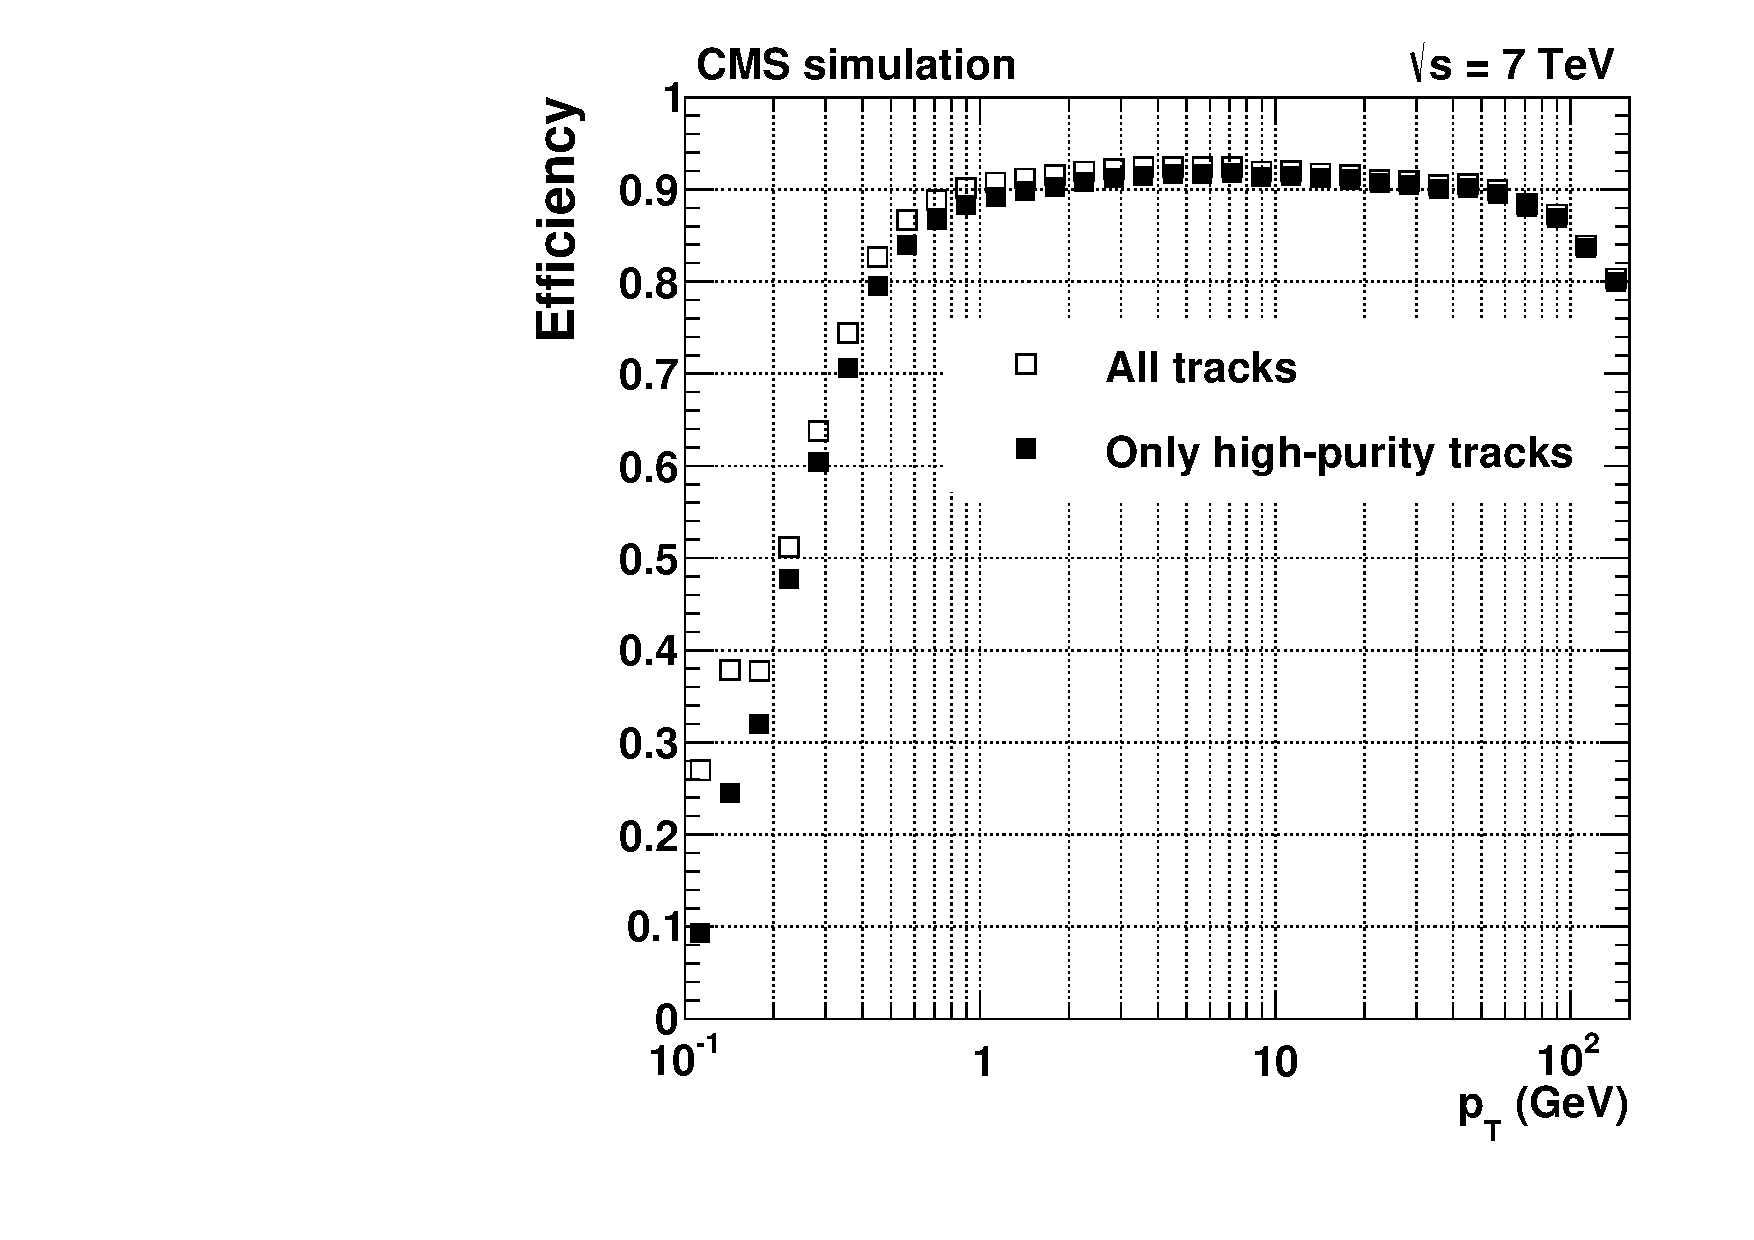
\includegraphics[width=0.65\textwidth]{figures/efficiencyVsPt.pdf}
    \caption[CMS integrated luminosity delivered and recorded over time.]{
      The integrated luminosity delivered to CMS over time by the LHC, in blue, and the portion CMS managed to record, in yellow.
      As can be seen, CMS is not 100% efficient at recording collisions. 
      It is important to note that this inefficiency is a straightforward failure to observe the events, {\it not} the purposeful rejection of events by the trigger system discussed in Section~\ref{sec:trigger}.
      Taken from \cite{lumipublic}.}
    \label{fig:intlumi}
  \end{figure}  


  The sensitivity of searches performed in CMS scales straightforwardly with the total number of collisions provided by the LHC.
  Thus far, the LHC has provided CMS with nearly 200~\fbinv across all operating periods, with the rate accelerating as the machine is pushed to the limits of its design, as shown in Figure~\ref{fig:intlumi}.
  The searches discussed in the next chapter use only the 137~\fbinv recorded by CMS during the 13~TeV runs from 2016 to 2018.
  As the total inelastic proton-proton collision cross section is approximately 69.2~mb at 13~TeV, the total number of collisions observed by CMS from 2016 to 2018 is nearly $10^{16}$.
  While this vast sample size makes very rare genuine physics processes potentially observable, it also presents a challenge in that very rare and difficult to model detector failures may pollute the dataset.
  It is prudent to adopt a conservative approach to any searches for rare new physics.

\section{The CMS Detector} \label{sec:CMS}

  While the LHC provides the collisions, it is the Compact Muon Solenoid (CMS) detector that ultimately measures the products and reconstructs each event.
  A detailed description of all of the CMS hardware and software is available in Reference~\cite{cms_tdr}, and a description of the general event reconstruction technique used at CMS, called Particle Flow, is available in Reference~\cite{particleflow}.
  This section serves as a general overview of how CMS works, sufficient to understand the searches for new physics presented later in this work.

  The particles stable enough to be detected directly by CMS come in 5 distinct varieties, namely electrons, muons, photons, charged hadrons (largely protons, pions, and charged kaons), and neutral hadrons (largely neutrons and neutral kaons).
  Figure~\ref{fig:cmsreconstruction} depicts a generic detection of each kind of particle.
  All other particles are too unstable to be measured directly, except the neutrinos.
  Neutrinos are, uniquely among Standard Model particles, both stable and invisible to CMS.
  Their presence in the products of a collision is inferred by measuring all of the visible content of an event, and noting that some energy is missing, as discussed in Section~\ref{sec:MET}.
  Any stable weakly interacting particles beyond the Standard Model produced in a collision at CMS would present a similar signature.

  \begin{figure}[h!]
    \centering
    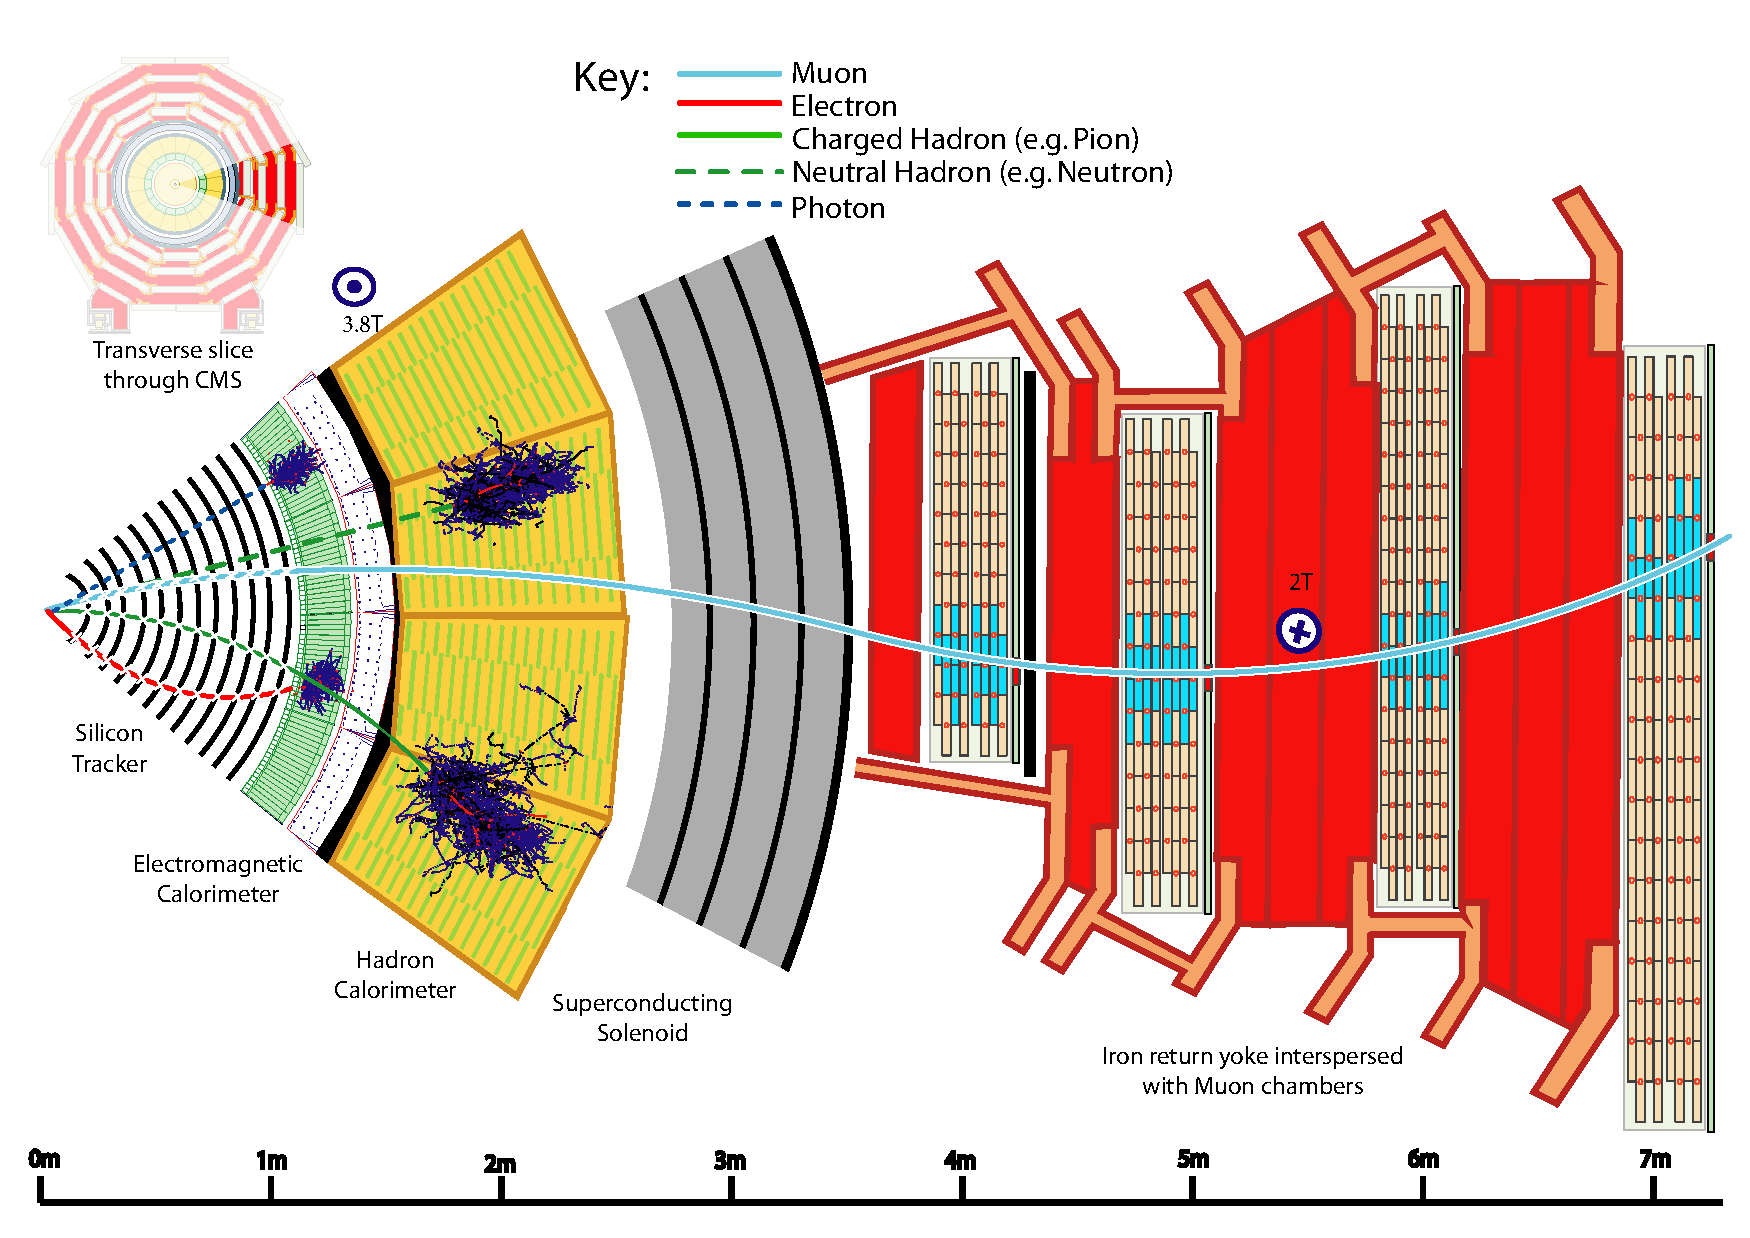
\includegraphics[width=0.85\textwidth]{figures/cmsreconstruction.pdf}
    \caption[Image depicting the experimental signatures of different types of particle at CMS.]{
      The design of CMS causes particles of different types to leave distinct experimental signatures, allowing them to be distinguished.
      The rest of this section references and explains this image.
      Taken from \cite{particleflow}.}
    \label{fig:cmsreconstruction}
  \end{figure}  

  The CMS detector is a cylinder composed of a central barrel section with two flat endcaps, each of which contain layers of different detection systems designed to provide the information necessary to distinguish the various particles that can be generated by collisions, and measure their positions and energies.
  Starting from the beam pipe, they are the tracker, the electromagnetic calorimeter, the hadronic calorimeter, and the muon system.
  The tracker and the calorimeters are inside a solenoid producing a magnetic field, while the muon system is subject only to the external, returning field of the solenoid.
  Altogether, the detector measures about 7.5 meters in radius and 21 meters in length.
  As suggested by the cylindrical detector shape, the experiment uses a cylindrical coordinate system, in which the beam axis is assigned to the z axis, and the angle in the transverse plane, $\phi$, is measured starting from a line connecting CMS to the center of the LHC ring.
  The trajectories of particles is often described using both this angle $\phi$ and the pseudorapidity $\eta$, 
  \begin{equation} \label{eqn:eta}
    \eta = \log\left[\tan\left(\frac{\theta}{2}\right)\right]
  \end{equation}
  where $\theta$ is the angle made with the z axis \cite{cmstdr}.
  This usage is motivated by the fact that the average flux of particles produced by collisions in a window of fixed $\Delta\eta=\eta_2-\eta_1$ is roughly constant for any $\eta_1$ and $\eta_2$.

  This section describes each of the subsystems, as well as the objects that are constructed using their measurements.

  \subsection{Magnet} \label{sec:magnet}

  As its name suggests, a major feature of the CMS detector is a superconducting solenoid, the largest ever built, which provides a constant 3.8~T magnetic field in the tracker and calorimeters.
  This magnetic field curves the trajectories of charged particles, allowing for a determination of their charges and assisting in the measurement of their masses and energies, contributing to highly accurate identification of particles.
  
  CMS is compact in part to make it possible to fit the bulk of the detector inside this single solenoid.
  This maximizes the strength and consistency of the magnetic field, which in turn maximizes the precision with which particle positions, and the curvatures of their trajectories, can be measured.

  In Figure~\ref{fig:cmsreconstruction}, one can see the path of an electron (orange) curving sharply, in a direction indicating that it is negatively charged.
  Similarly, the path of a charged hadron (solid green) curves in the opposite direction, indicating a positive charge.
  A positively charged muon (blue) curves first one way, then the reverse once the field flips after exiting the solenoid.
  Neutral particles (dotted lines) do not curve at all.

  \subsection{Tracker} \label{sec:tracker}

  The silicon tracker is the innermost detector system and is primarily responsible for measuring the positions of charged particles.  
  In Figure~\ref{fig:cmsreconstruction}, the trajectories of neutral particles are represented with dotted lines, to indicate that they do not actually leave those tracks in the detector.
  The tracker is critically important for the disappearing tracks search covered in Section~\ref{sec:distracks}, and so is described here in more detail than the other detector systems.

  \begin{figure}[h!]
    \centering
    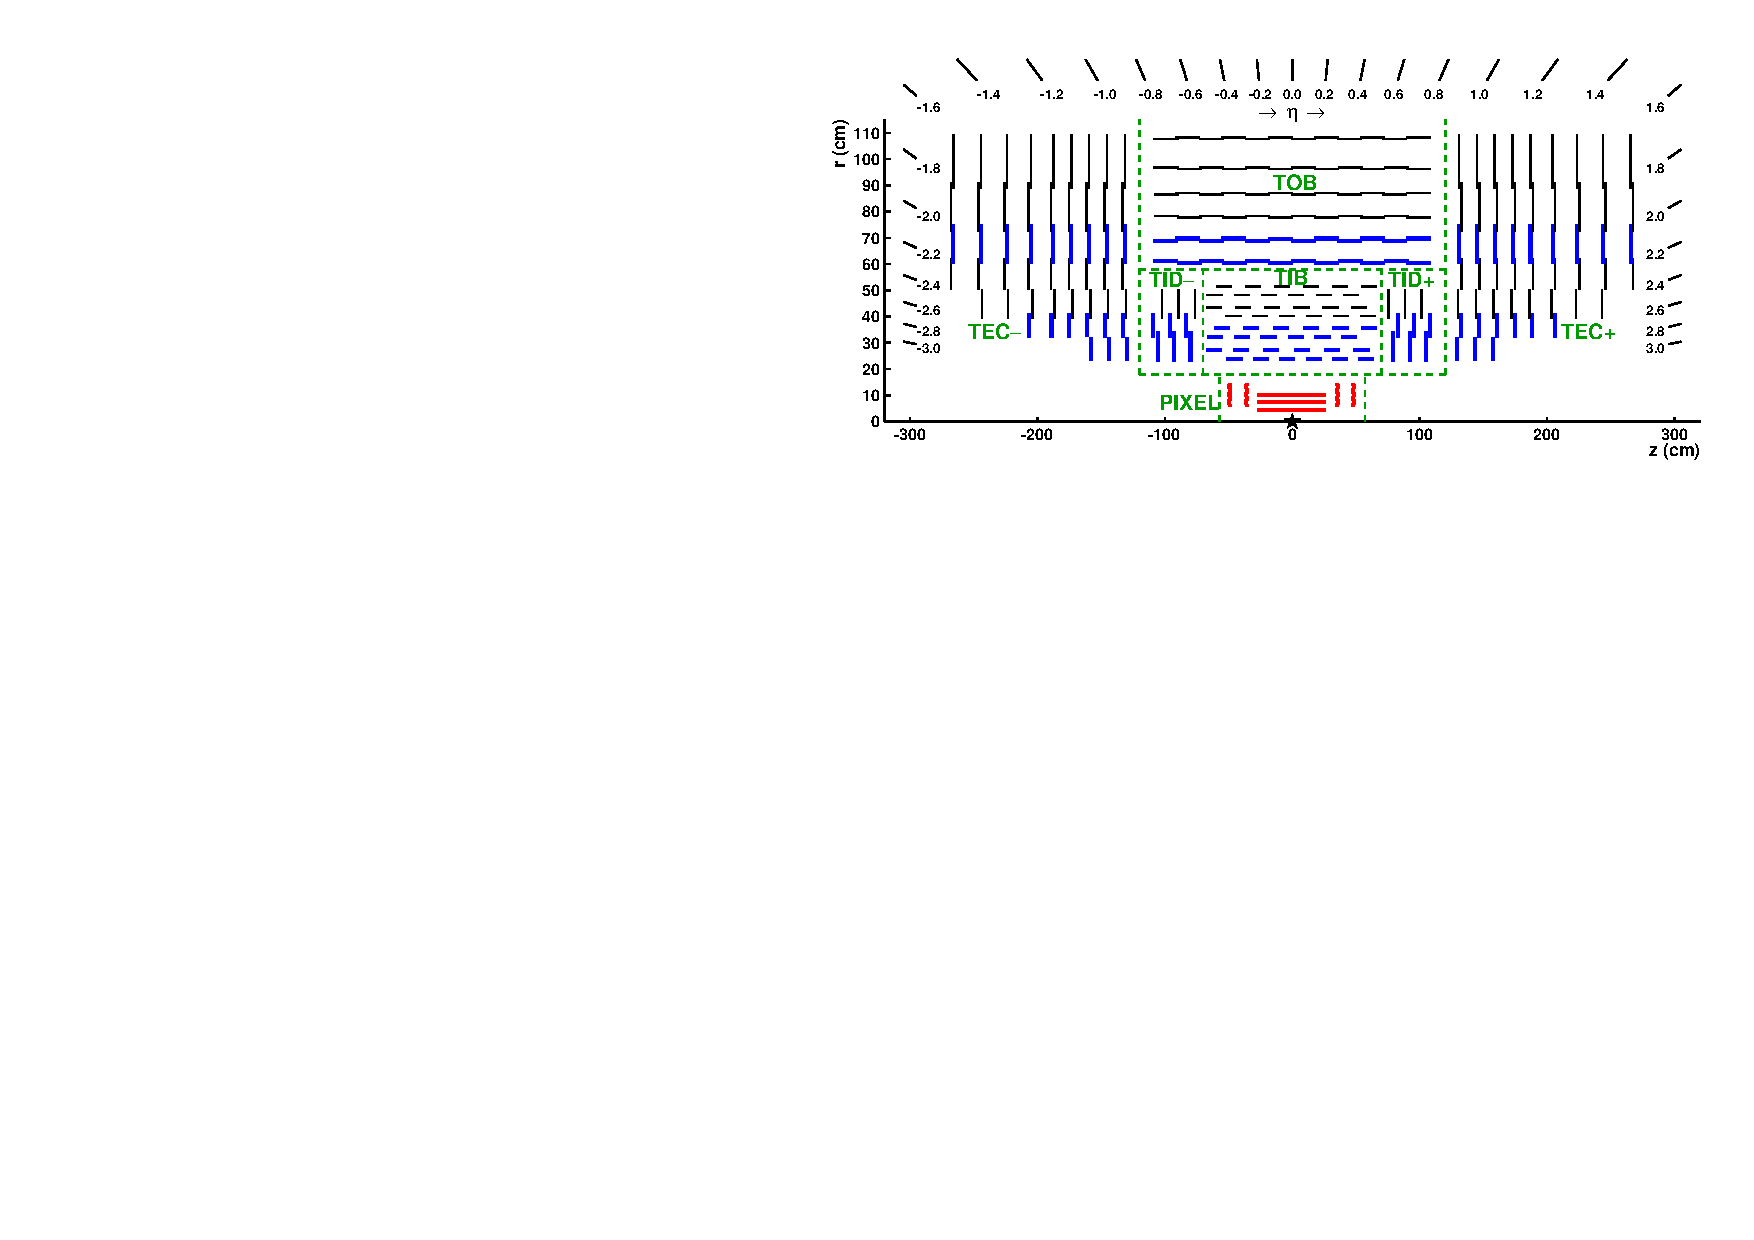
\includegraphics[width=0.75\textwidth]{figures/TrackerLayout.pdf}
    \caption[Layout of the tracker up to 2016.]{
      A slice of the CMS tracker in the $r-z$ plane, with the inner pixel tracker (red) in the 3-layer configuration used until 2016.
      In 2017 and 2018, the pixel tracker was upgraded with a 4th layer.
      The tracker is symmetric about the beam axis ($r=0$); one should imagine rotating this image around the horizontal axis to form a cylinder, to visualize the tracker's 3-dimensional form.
      The labels in green text denote tracker subsystems, the Tracker End Cap, the Tracker Inner Disk, the Pixel Tracker, the Tracker Inner Barrel, and Tracker Outer Barrel.
      The interior subsystems have more miniaturized detector elements and, therefore, better resolution.
      Taken from \cite{cmstracking}.}
    \label{fig:trackerlayout}
  \end{figure}  

  \begin{figure}[h!]
    \centering
    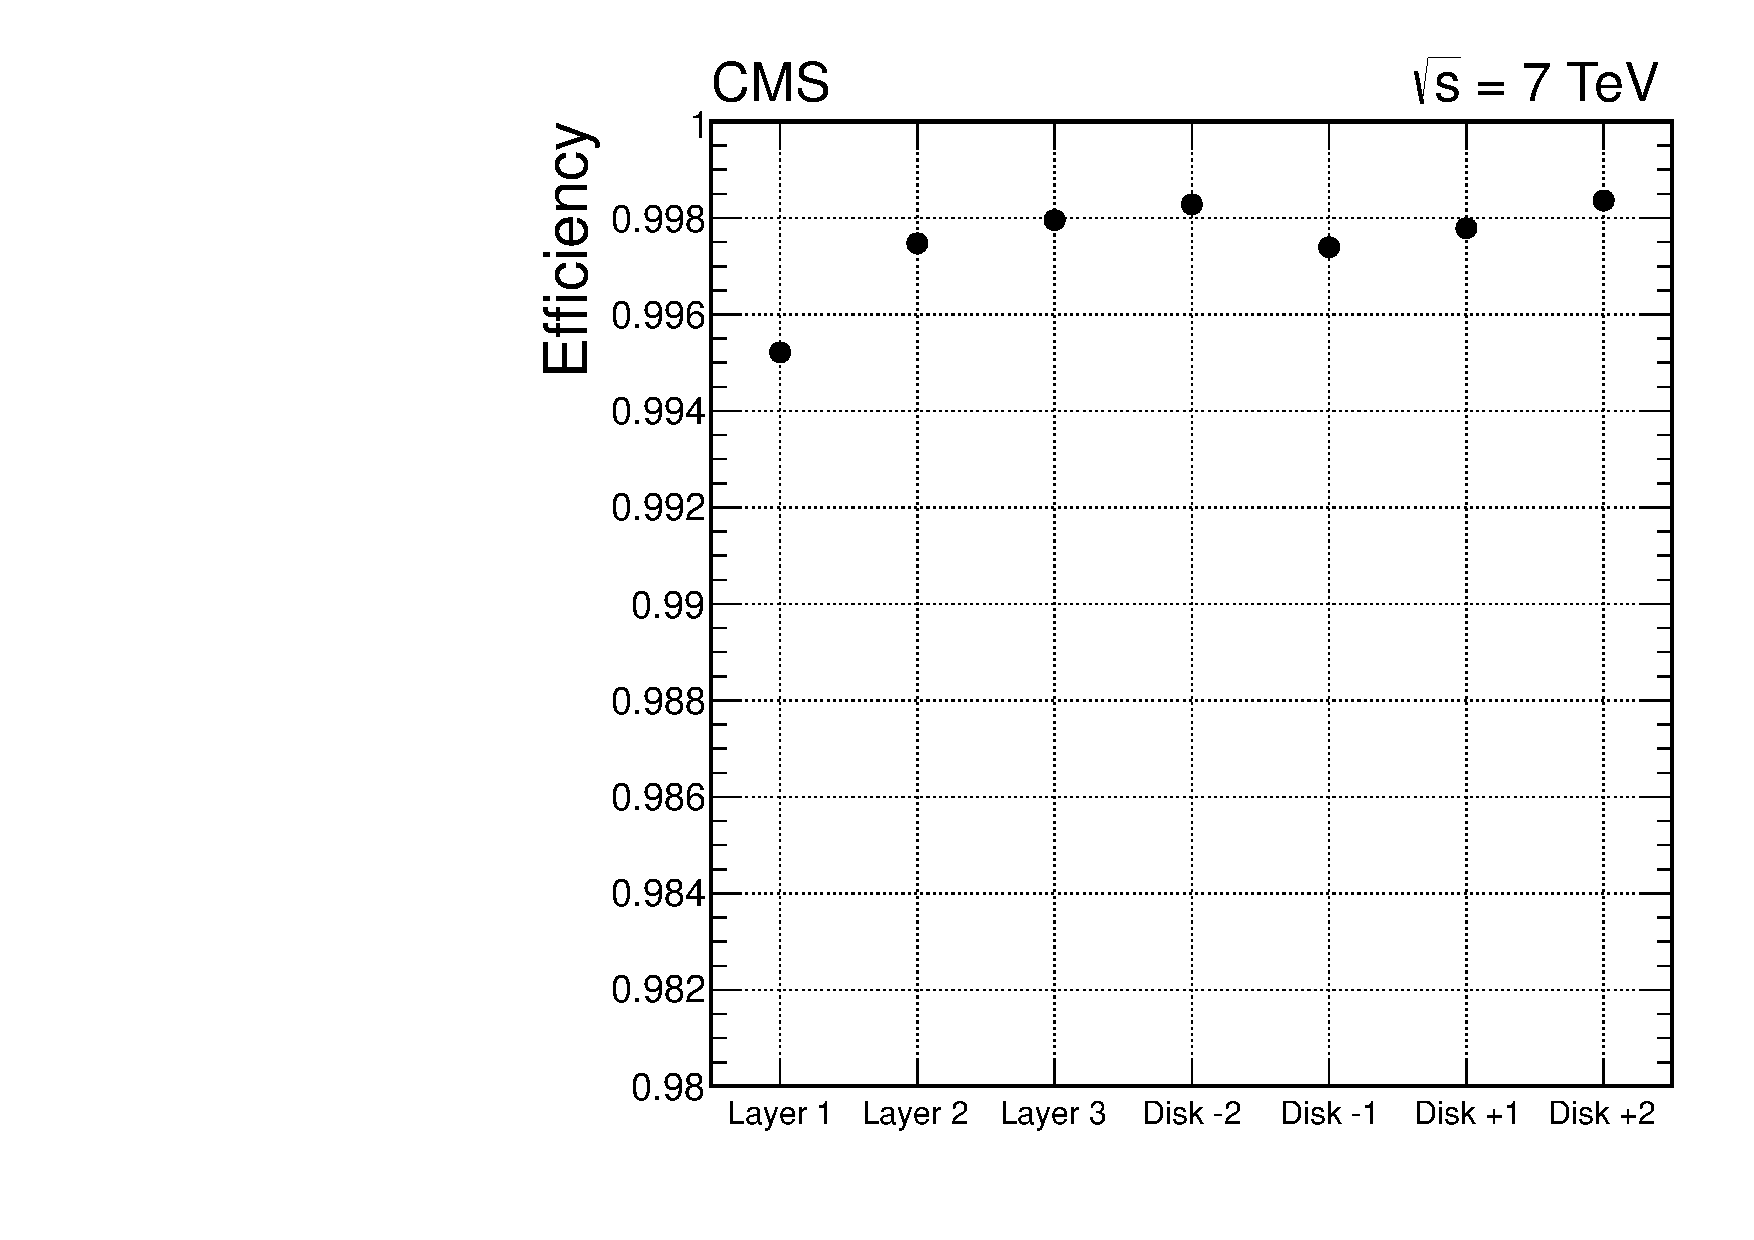
\includegraphics[width=0.65\textwidth]{figures/hitefficiency.pdf}
    \caption[Efficiency for a genuine particle to leave an expected hit in the CMS tracker.]{
      The efficiency for a genuine charged particle to produce an expected hit in the various components of the CMS pixel tracker, in the configuration used in 2016 and earlier. 
      Fake tracks may have many missing expected hits, but more than one or perhaps two is extremely rare in tracks produced by genuine particles.
      The probability for a neutral particle to produce a hit is small, and the probability to leave enough to produce a track is negligible.
      Taken from \cite{cmstracking}.}
    \label{fig:hitefficiency}
  \end{figure}  

  As shown in Figure~\ref{fig:trackerlayout}, the tracker is composed of several discrete layers.
  When a charged particle passes through a layer, it usually causes a measurable current to flow in the silicon, and is said to have produced a ``hit.''  
  As shown in Figure~\ref{fig:hitefficiency}, the probability for a genuine particle to leave a hit is near but not quite unity, so a missing hit where one would be expected is credible but cause for skepticism.
  Each event produces an intimidating array of these discrete hits throughout the tracker, which must then be connected by the track reconstruction algorithm into particle tracks.
  CMS uses an iterative procedure described in Reference~\cite{cmstracking}, in which clean, high energy, isolated tracks are reconstructed first so that their hits may be removed from the pool, followed by the next most obvious tracks, and so on, dramatically simplifying the computational complexity of each step.
  The early iterations that produce the tracks judged to be of highest quality find only those tracks with transverse momenta at least 0.3~GeV, and no iteration can produce a track with transverse momentum below 0.1~GeV, so that particles of such low energy are effectively invisible to CMS.
  Note that, due to the strong magnetic field present in the tracker, particles with energies lower than around 0.1 GeV travel in such tight spirals that reconstruction becomes infeasible.
  Although this is normally insignificant, since these particles are not typically important to an event's overall characterization, this fact allows for the existence of disappearing tracks, in which a high energy charged particle decays to a trackless neutral particle and a charged particle of such low energy that it is not reconstructed.
  Additionally, all tracks must be composed of at least 3 hits.

  The performance is outstanding, especially for tracks passing the sophisticated ``high purity'' selection applied by the vast majority of CMS analyses. 
  Figure~\ref{fig:trackfakerate} shows the fake rate of this procedure, less than 5\% for tracks in the intermediate energy range, and further suppressible with additional cleaning selections like those of the disappearing tracks search covered in Section~\ref{sec:distracks}.
  Figure~\ref{fig:trackefficiency} shows the efficiency to reconstruct tracks successfully for the three most common varieties of charged particles measured by CMS, namely muons (left), electrons (center), and pions (right), approaching unity in all cases for higher energy tracks in the barrel region of the tracker.

  \begin{figure}[h!]
    \centering
    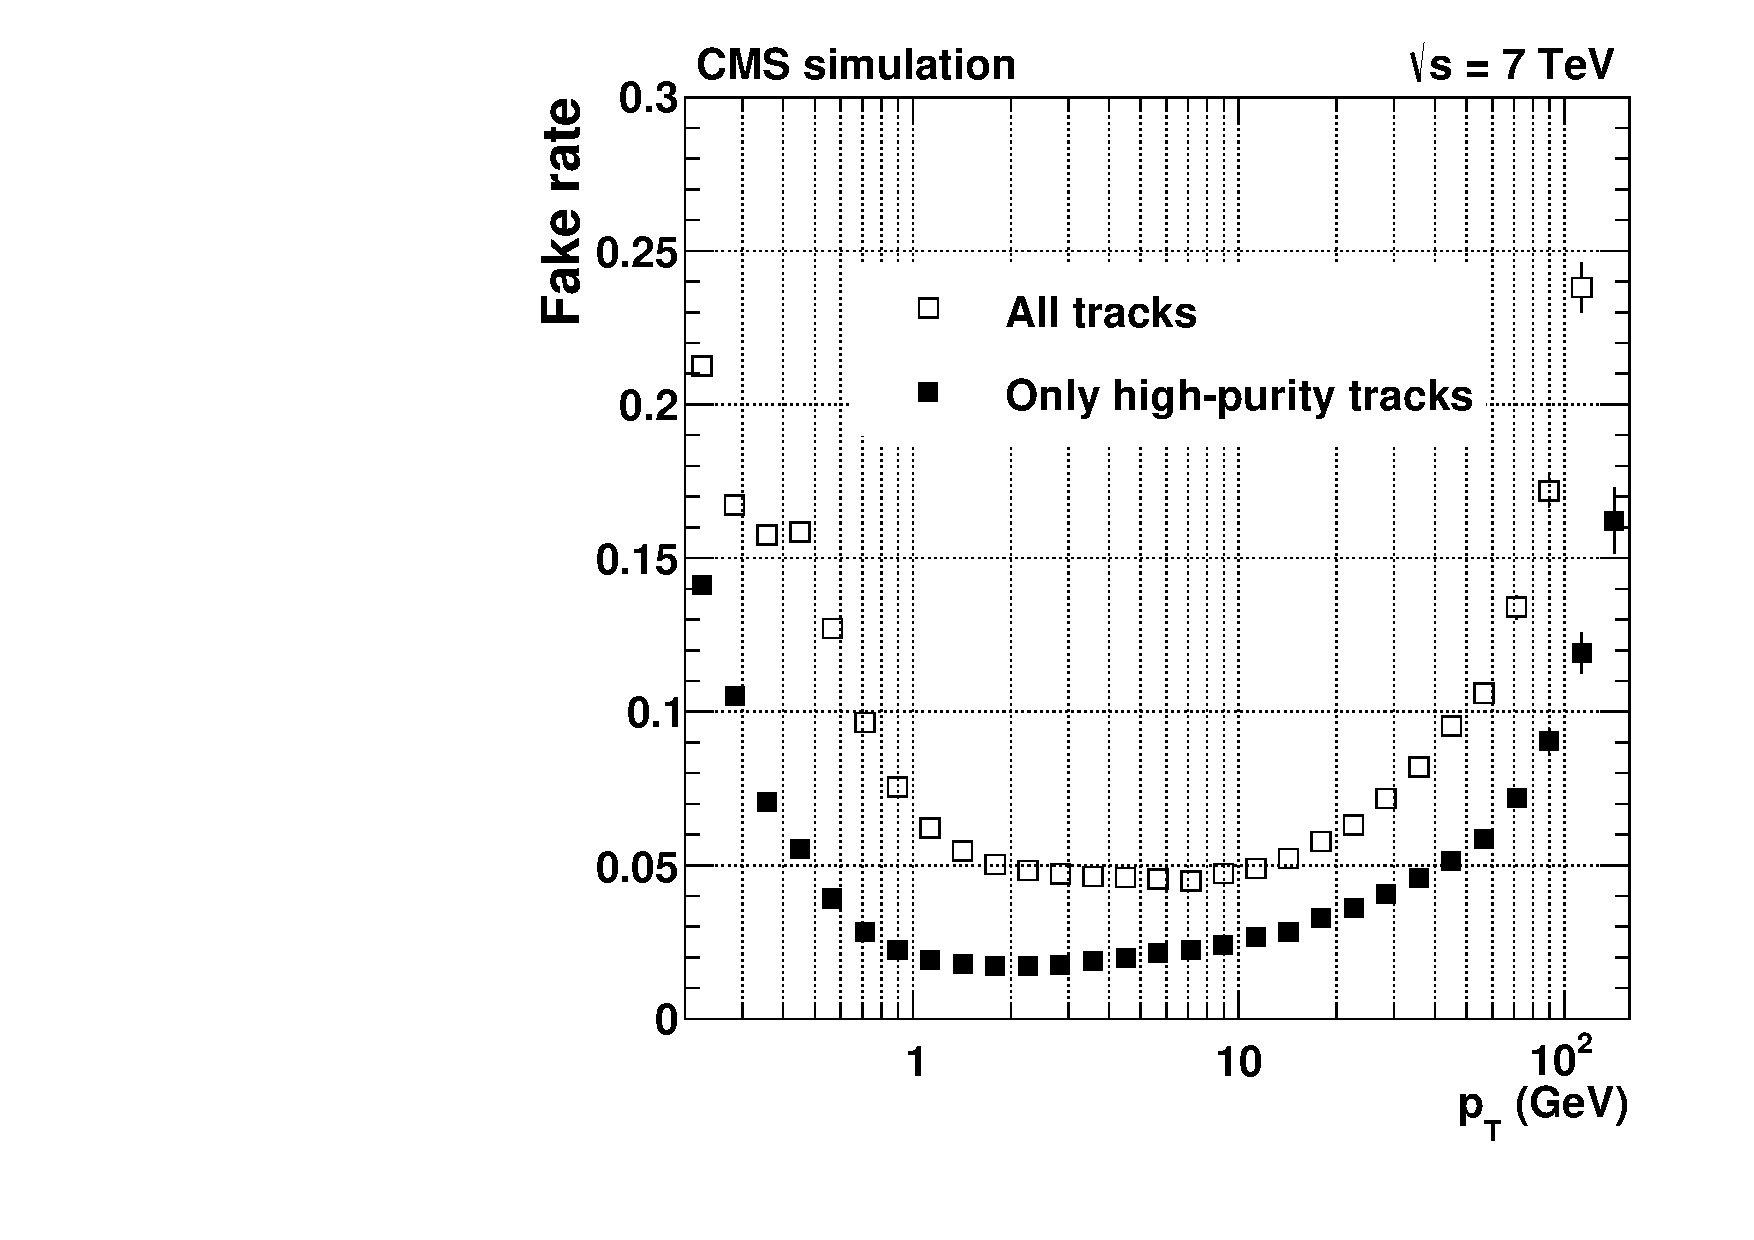
\includegraphics[width=0.65\textwidth]{figures/fakerateVsPt.pdf}
    \caption[Track fake rate.]{
      The CMS track fake rate as a function of \pt, in the configuration used in 2016 and earlier. 
      The sophisticated high purity selection aims to suppress the fake rate without badly affecting efficiency and is applied in the vast majority of CMS analyses. 
      Taken from \cite{cmstracking}.}
    \label{fig:trackfakerate}
  \end{figure}  

  \begin{figure}[h!]
    \centering
    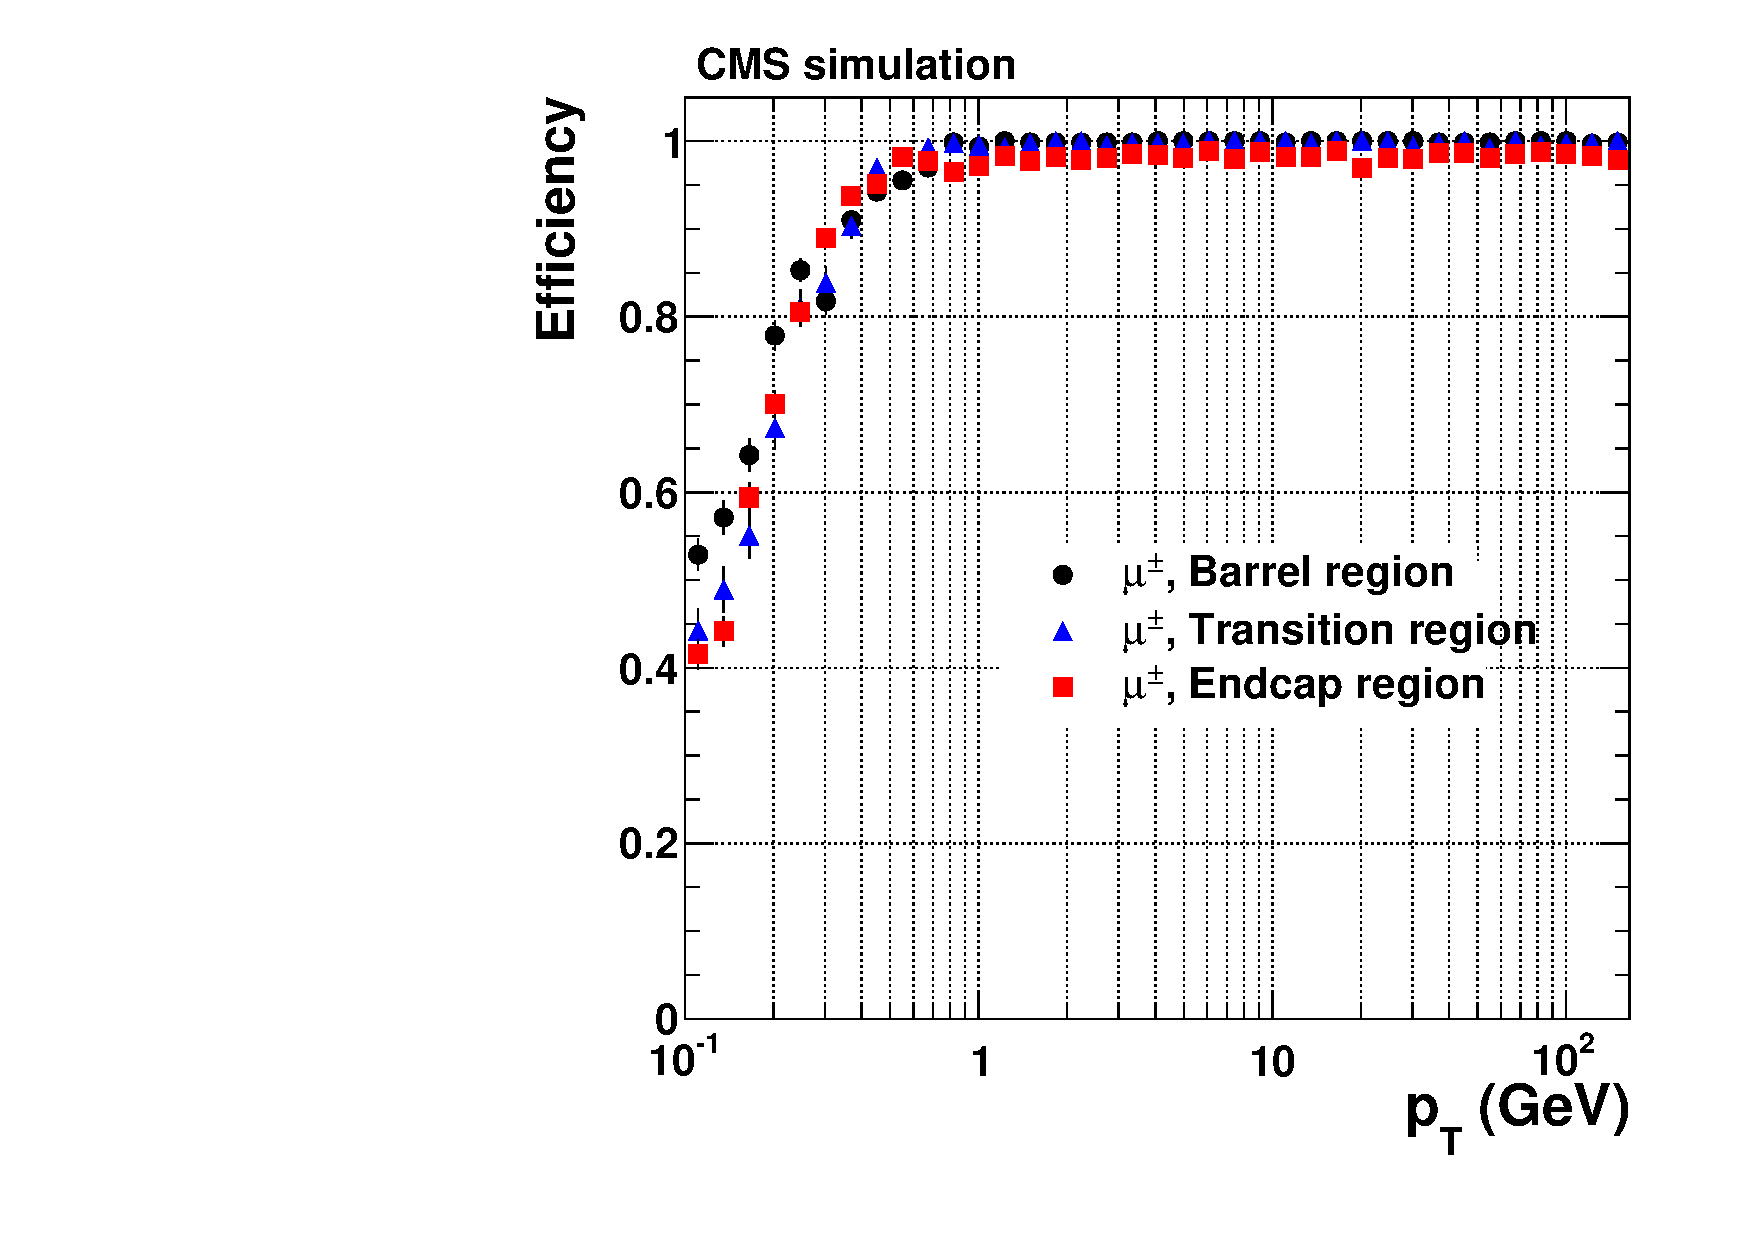
\includegraphics[width=0.3\textwidth]{figures/mu/efficiencyVsPt.pdf}
    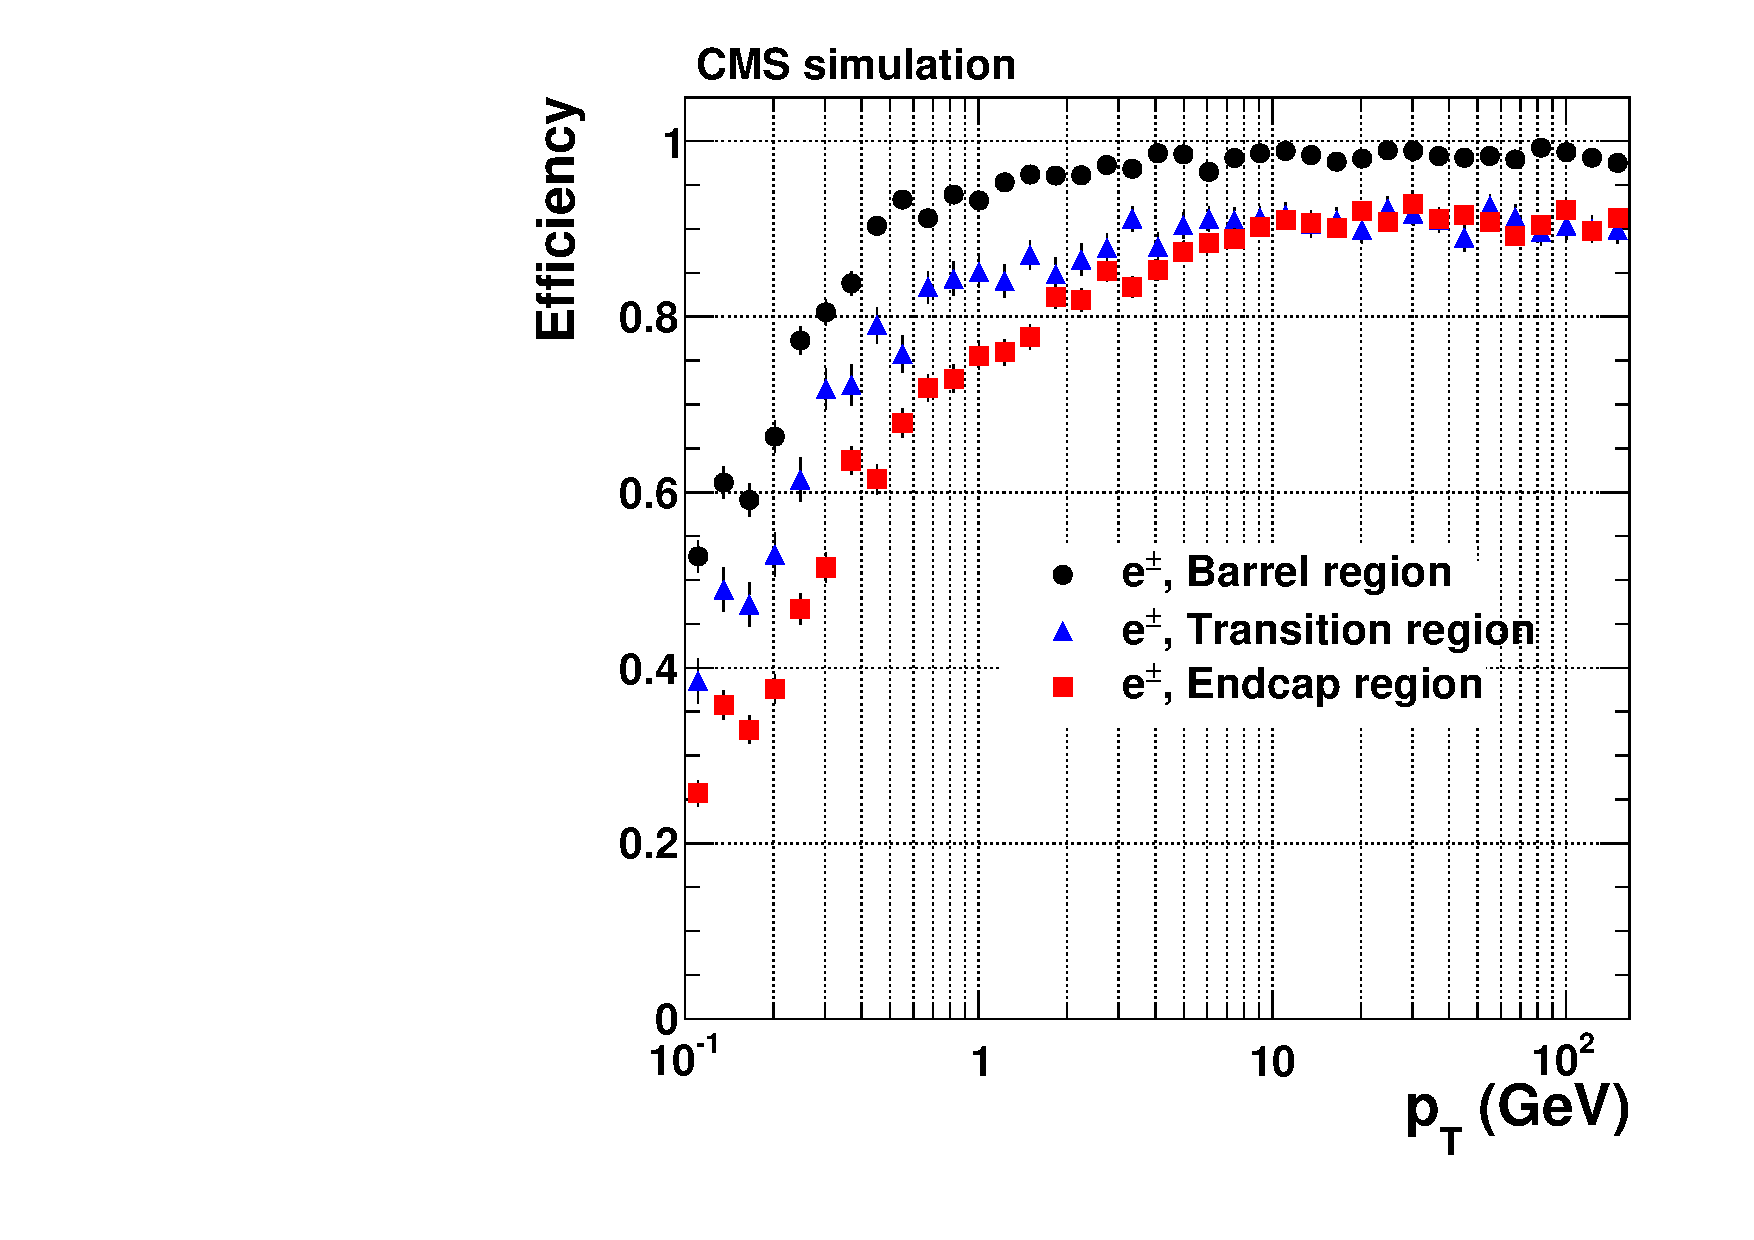
\includegraphics[width=0.3\textwidth]{figures/el/efficiencyVsPt.pdf}
    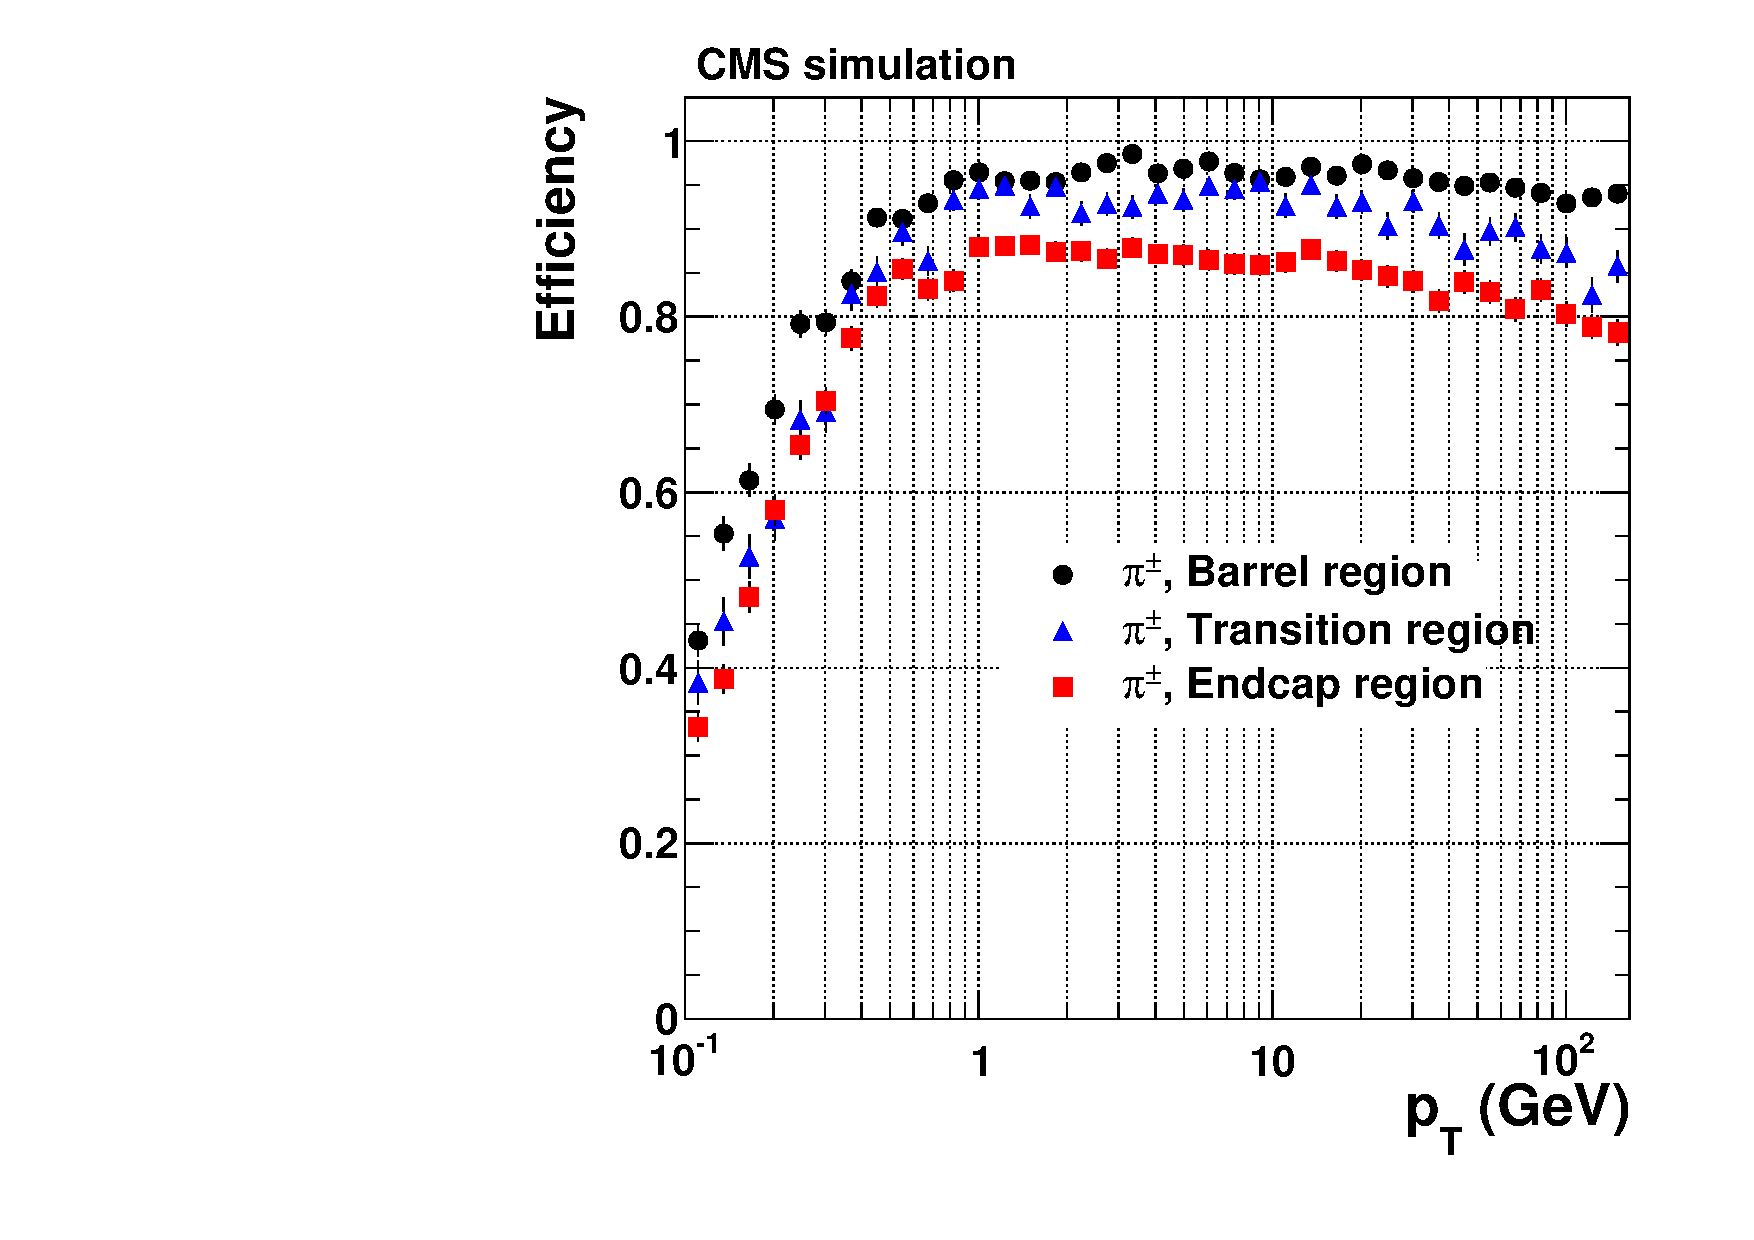
\includegraphics[width=0.3\textwidth]{figures/pi/efficiencyVsPt.pdf}
    \caption[Track reconstruction efficiency.]{
      The CMS track reconstruction efficiency for (left) muons, (center) electrons, and (right) pions, split by detector region as a function of \pt, in the configuration used in 2016 and earlier. 
      Muons are by far the cleanest objects at CMS as they are massive enough to avoid strong perturbations by tracker material, and lack nuclear interactions.
      Electrons are lighter and so are vulnerable to tracker interactions, experiencing strong bremsstrahlung losses, while pions can undergo nuclear interactions.
      Taken from \cite{cmstracking}.}
    \label{fig:trackefficiency}
  \end{figure}  

  \begin{figure}[h!]
    \centering
    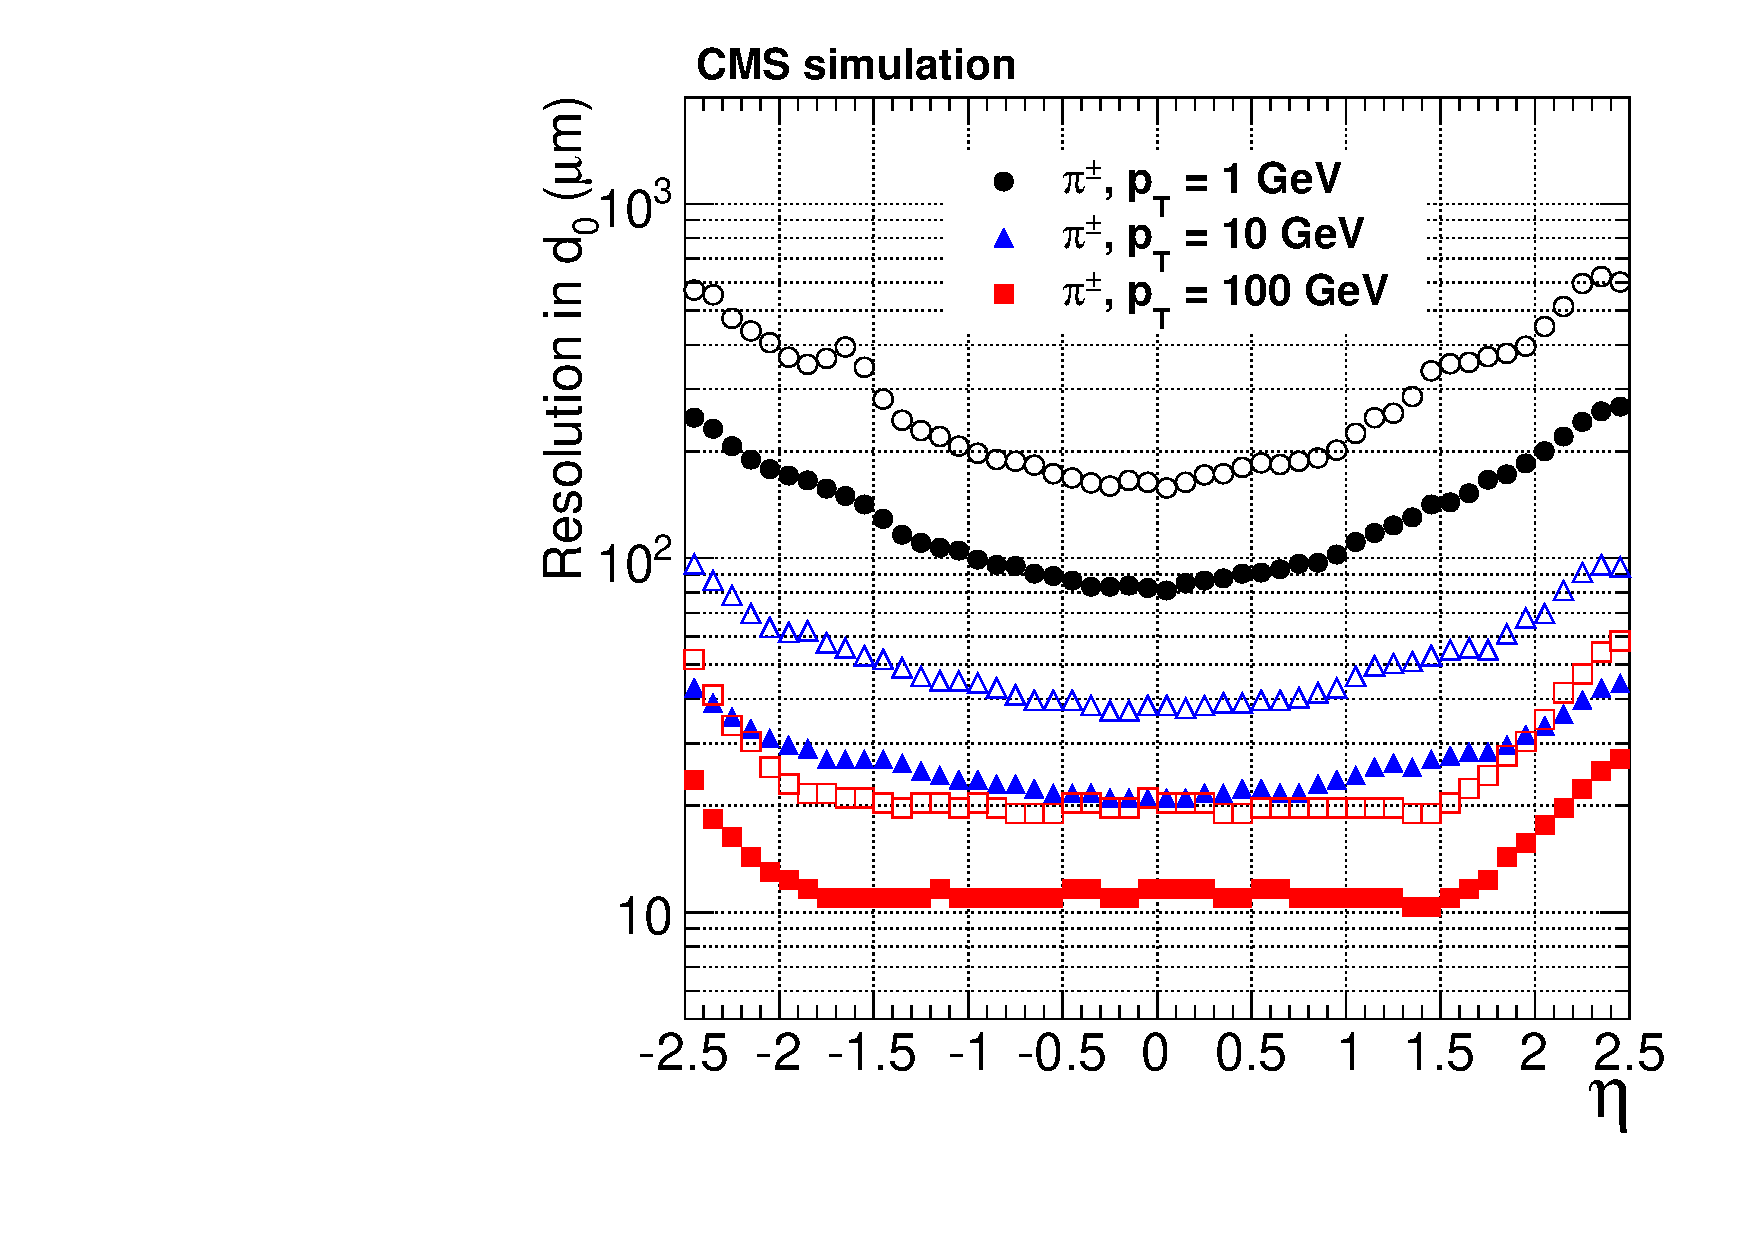
\includegraphics[width=0.4\textwidth]{figures/pi/resolutionD0VsEta.pdf}
    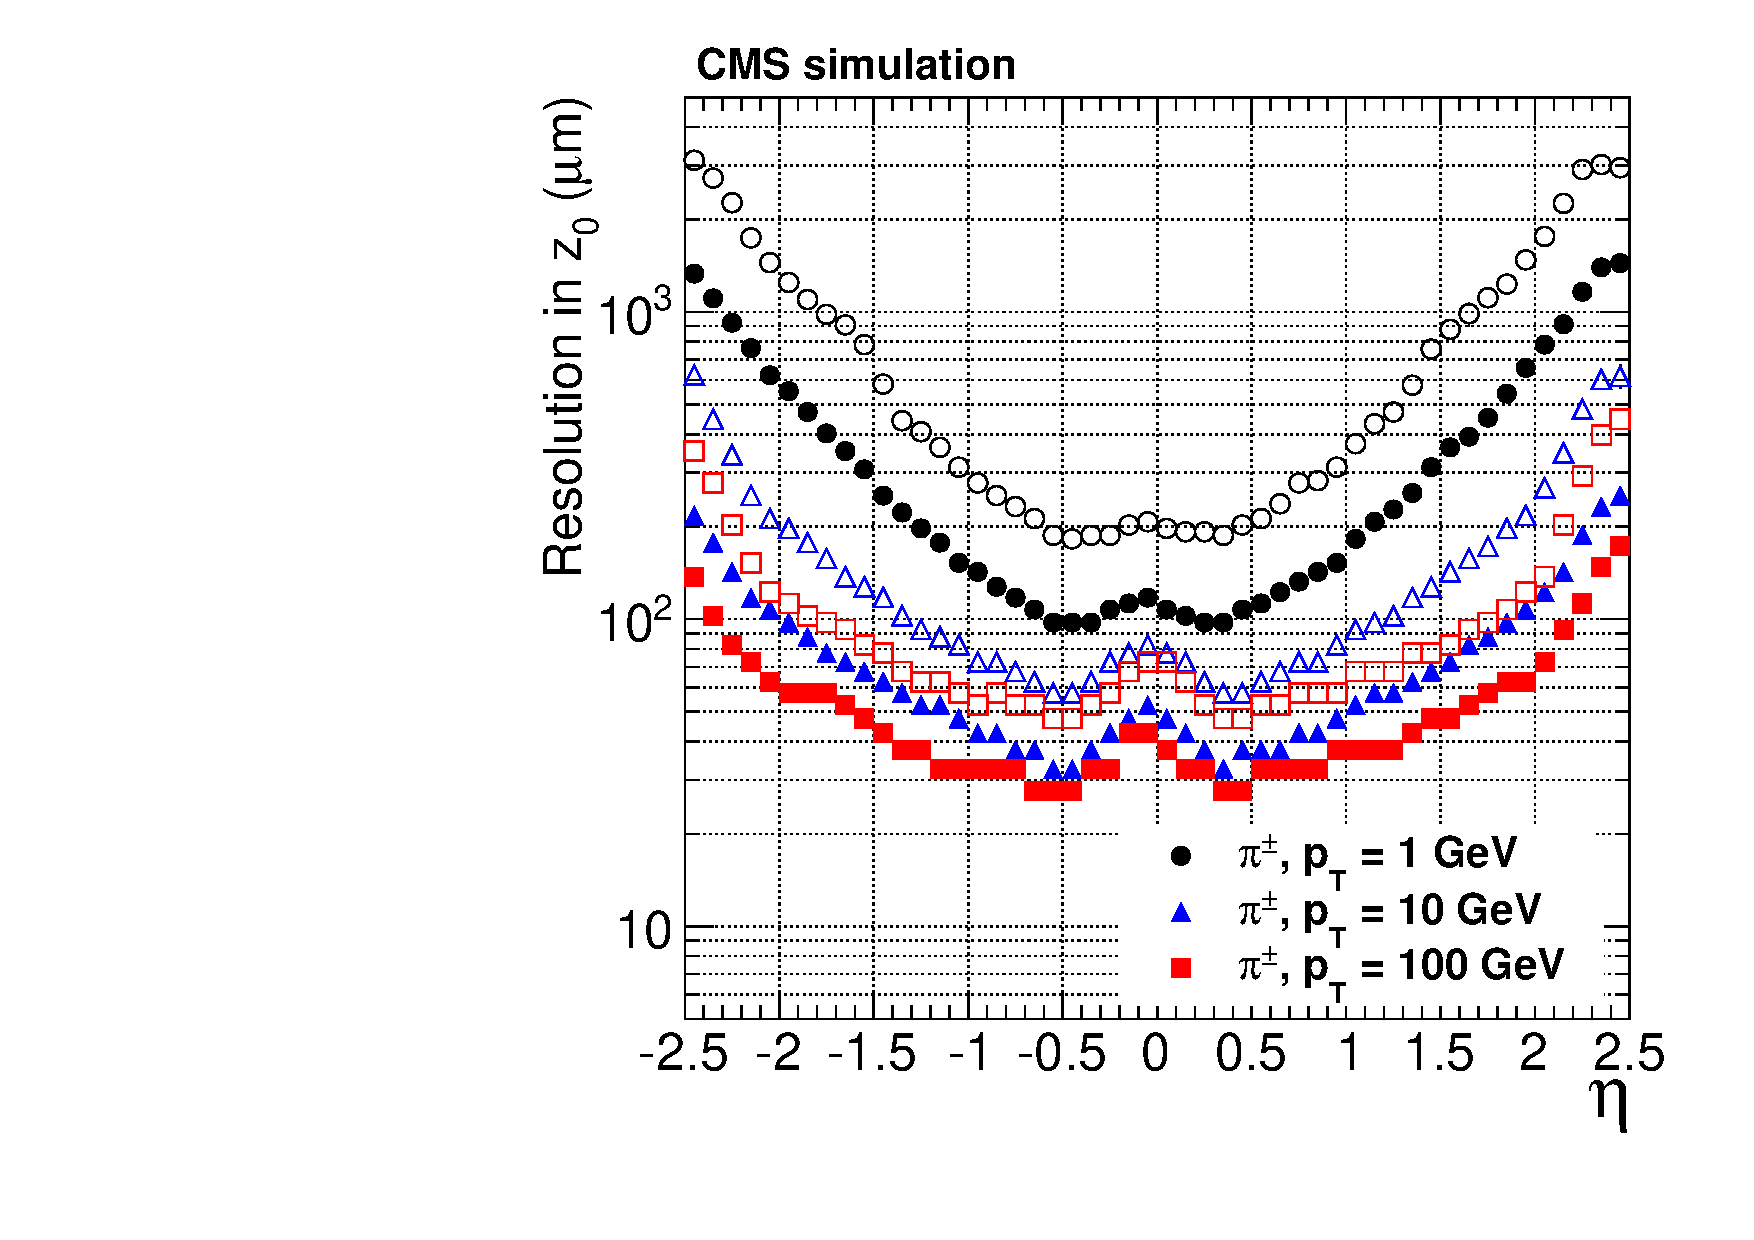
\includegraphics[width=0.4\textwidth]{figures/pi/resolutionDzVsEta.pdf}
    \caption[Impact parameter resolution in the CMS tracker.]{
      The CMS tracker has micron-level impact parameter resolution, for both (left) the transverse plane and (right) the z direction.
      Solid markers indicate the half-width of the 68\% confidence interval, while open markers indicate 90\% confidence.
      With this resolution, a track reconstructed with an impact parameter of more than a few hundred microns is likely a fake, from a pileup vertex, or from a secondary vertex produced by a decaying particle like a bottom hadron.
      Taken from \cite{cmstracking}.}
    \label{fig:trackresolution}
  \end{figure}  

  The tracker detection elements are smaller and consequently provide better localization in interior layers of the tracker, with the pixel detector components only approximately 100 $\mu$m across.
  As a general guideline, no element in the tracker is permitted to have an expected probability of a hit greater than 1\% per bunch crossing, to maintain a low probability of tracks intersecting.
  This structure produces outstanding sub-millimeter resolution of a track's origin, shown in Figure~\ref{fig:trackresolution}, allowing tracks originating from collisions only microns apart to be separated, and tracks originating from decays of particles with decay lengths on the order of a millimeter to be identified.
  The former is important for rejection of pileup, and the latter for identification of jets originating from bottom quark hadrons.

    \subsubsection{Vertices and b-Tagging} \label{sec:btagging}

    Almost every track ultimately originates from a single point in a proton-proton collision.
    Tracks reconstructed in the tracker can be extrapolated back to their origins to form vertices, locations at which multiple tracks intersect and the inferred location of the initial hard interaction between partons.
    All the content associated with a single vertex constitutes a single event, subject to analysis in an attempt to determine the nature of the physics that occurs in the hard interactions

    Some tracks do not extrapolate to a proton-proton primary vertex back but instead a point a few millimeters away.
    While a few millimeters is not even enough to exit the beam pipe, such a decay length is nevertheless well within the tracker's resolution.
    These features are called secondary vertices, and are a distinctive feature of jets associated with hadrons containing bottom quarks.
    These hadrons, uniquely, have decay lengths on the order of millimeters.
    Charmed hadrons tend to decay somewhat more quickly, while hadrons containing only up, down, and strange quarks tend to live long enough to reach the calorimeters.
    These secondary vertices, along with some other indicators including the muon content of a jet, the number of tracks, and the mass, are leveraged bysophisticated algorithms that can identify jets originating from bottom quarks produced in the hard process with high efficiency \cite{btagging}.
    Such jets are said to be ``b-tagged.''
    The fake rate for a given efficiency achieved by various b-tagging algorithms is shown in Figure~\ref{fig:btageff}, with the older algorithms listed first and the newer, machine learning-based algorithms last.
    The analyses discussed in Section~\ref{analysis} apply the DeepCSV algorithm (purple) at the 1\% light quark fake rate working point, which achieves a successful b-tag rate of nearly 70\% and a charm quark mistag rate of just over 10\%.

  \begin{figure}[h!]
    \centering
    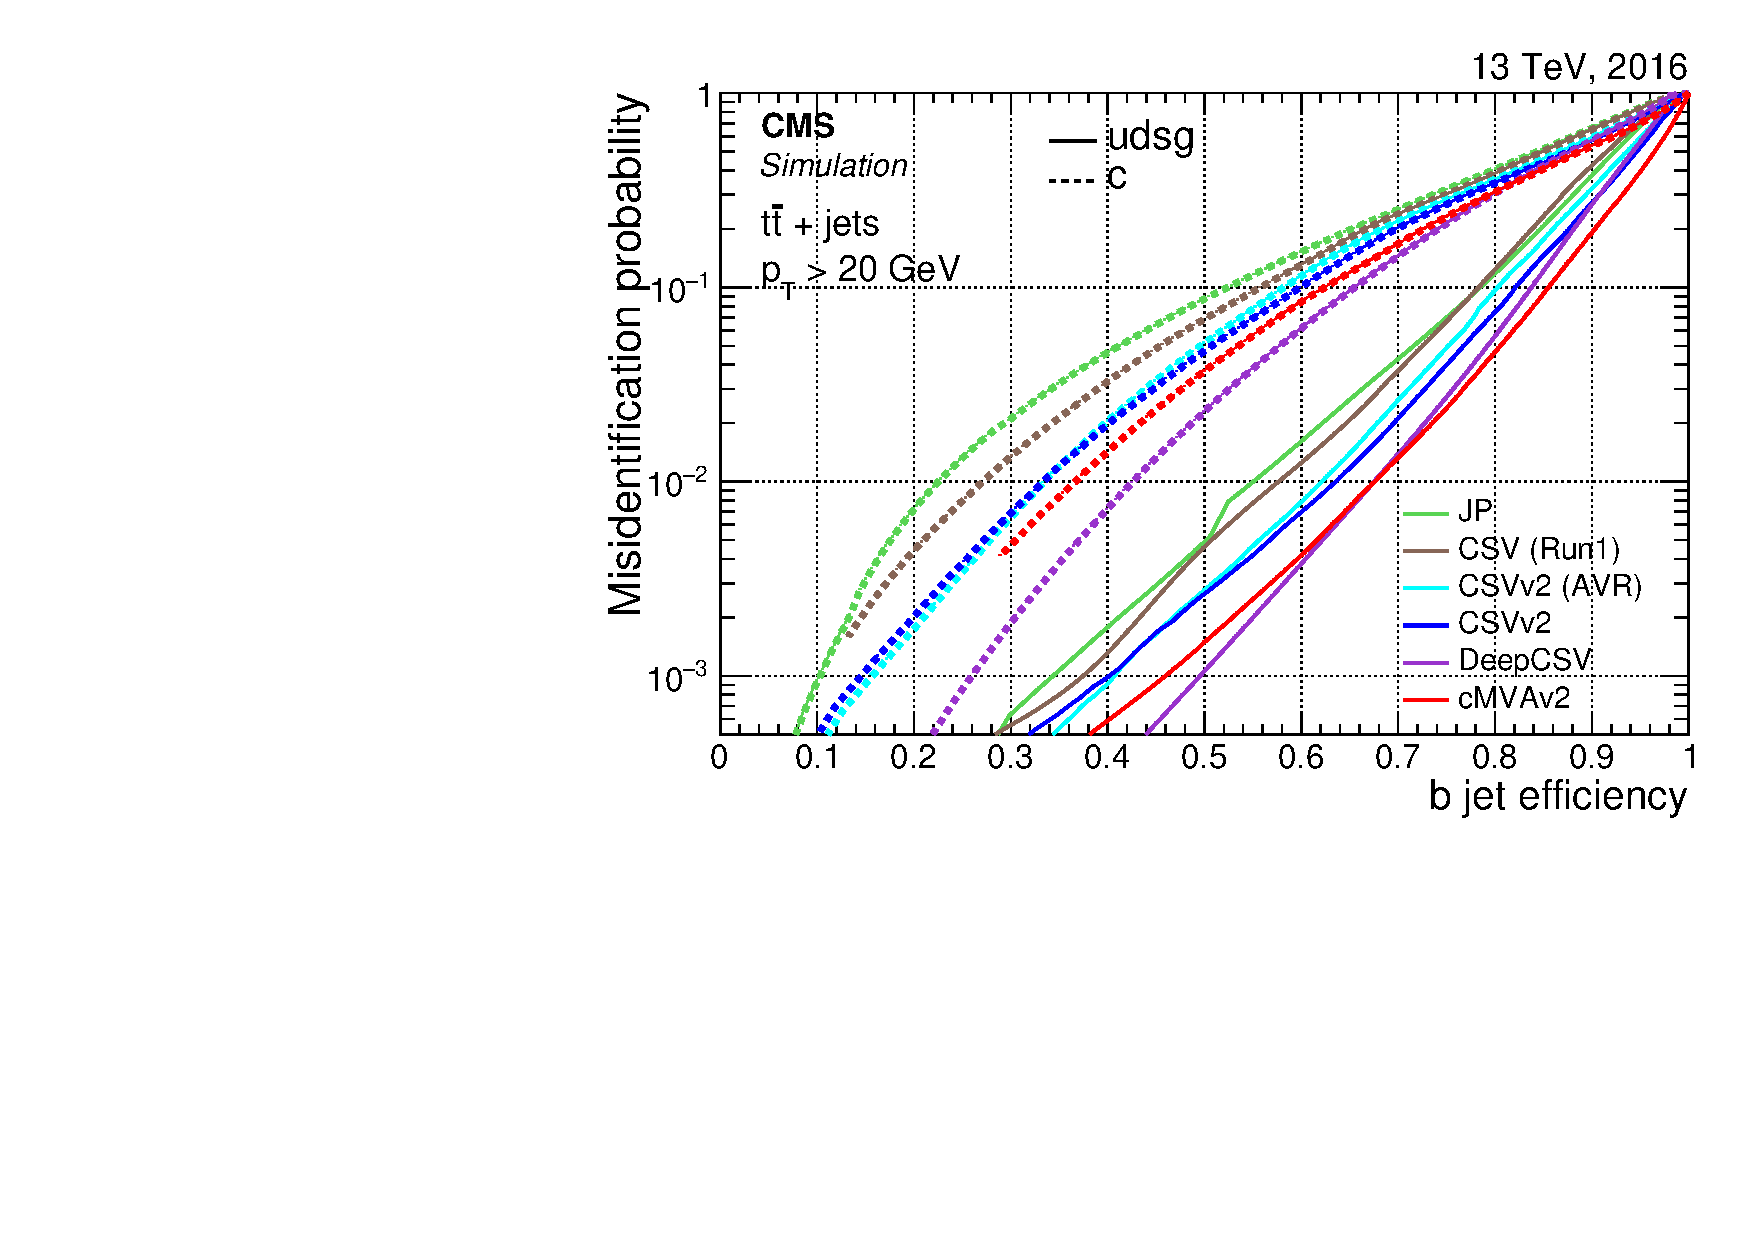
\includegraphics[width=0.65\textwidth]{figures/btageff.pdf}
    \caption[Efficiency and fake-rates of various b-tagging algorithms.]{
      The fake rate of various b-tagging algorithms (different colored lines) are plotted against the successful tag rate for genuine b-jets.
      Although charm quarks are distinguishable from bottom quarks in a variety of ways, including shorter lifetimes, they are still similar enough to cause a meaningful fake rate.
      These curves are plotted as dotted lines.
      The lighter quark fake rate is much lower, shown as solid lines.
      The algorithm of most interest is DeepCSV, a machine learning algorithm used in the analyses discussed in Section~\ref{analysis}.
      Taken from \cite{btagging}.}
    \label{fig:btageff}
  \end{figure}  

  Although the ability to identify a jet's source flavor is intrinsically useful, the identification of bottom quarks is of special interest because they tend appear in the majority of Higgs and top quark decays, and for their relative rarity in generic QCD multijet events compared to lighter quark flavors, which means that requiring many b-tags greatly suppresses background.
  Supersymmetry searches consider the case of bottom and top superpartners separately due in large part to the number of b-jets expected in the final state, and the consequently different, smaller backgrounds that dominate these models.

  \begin{figure}[h!]
    \centering
    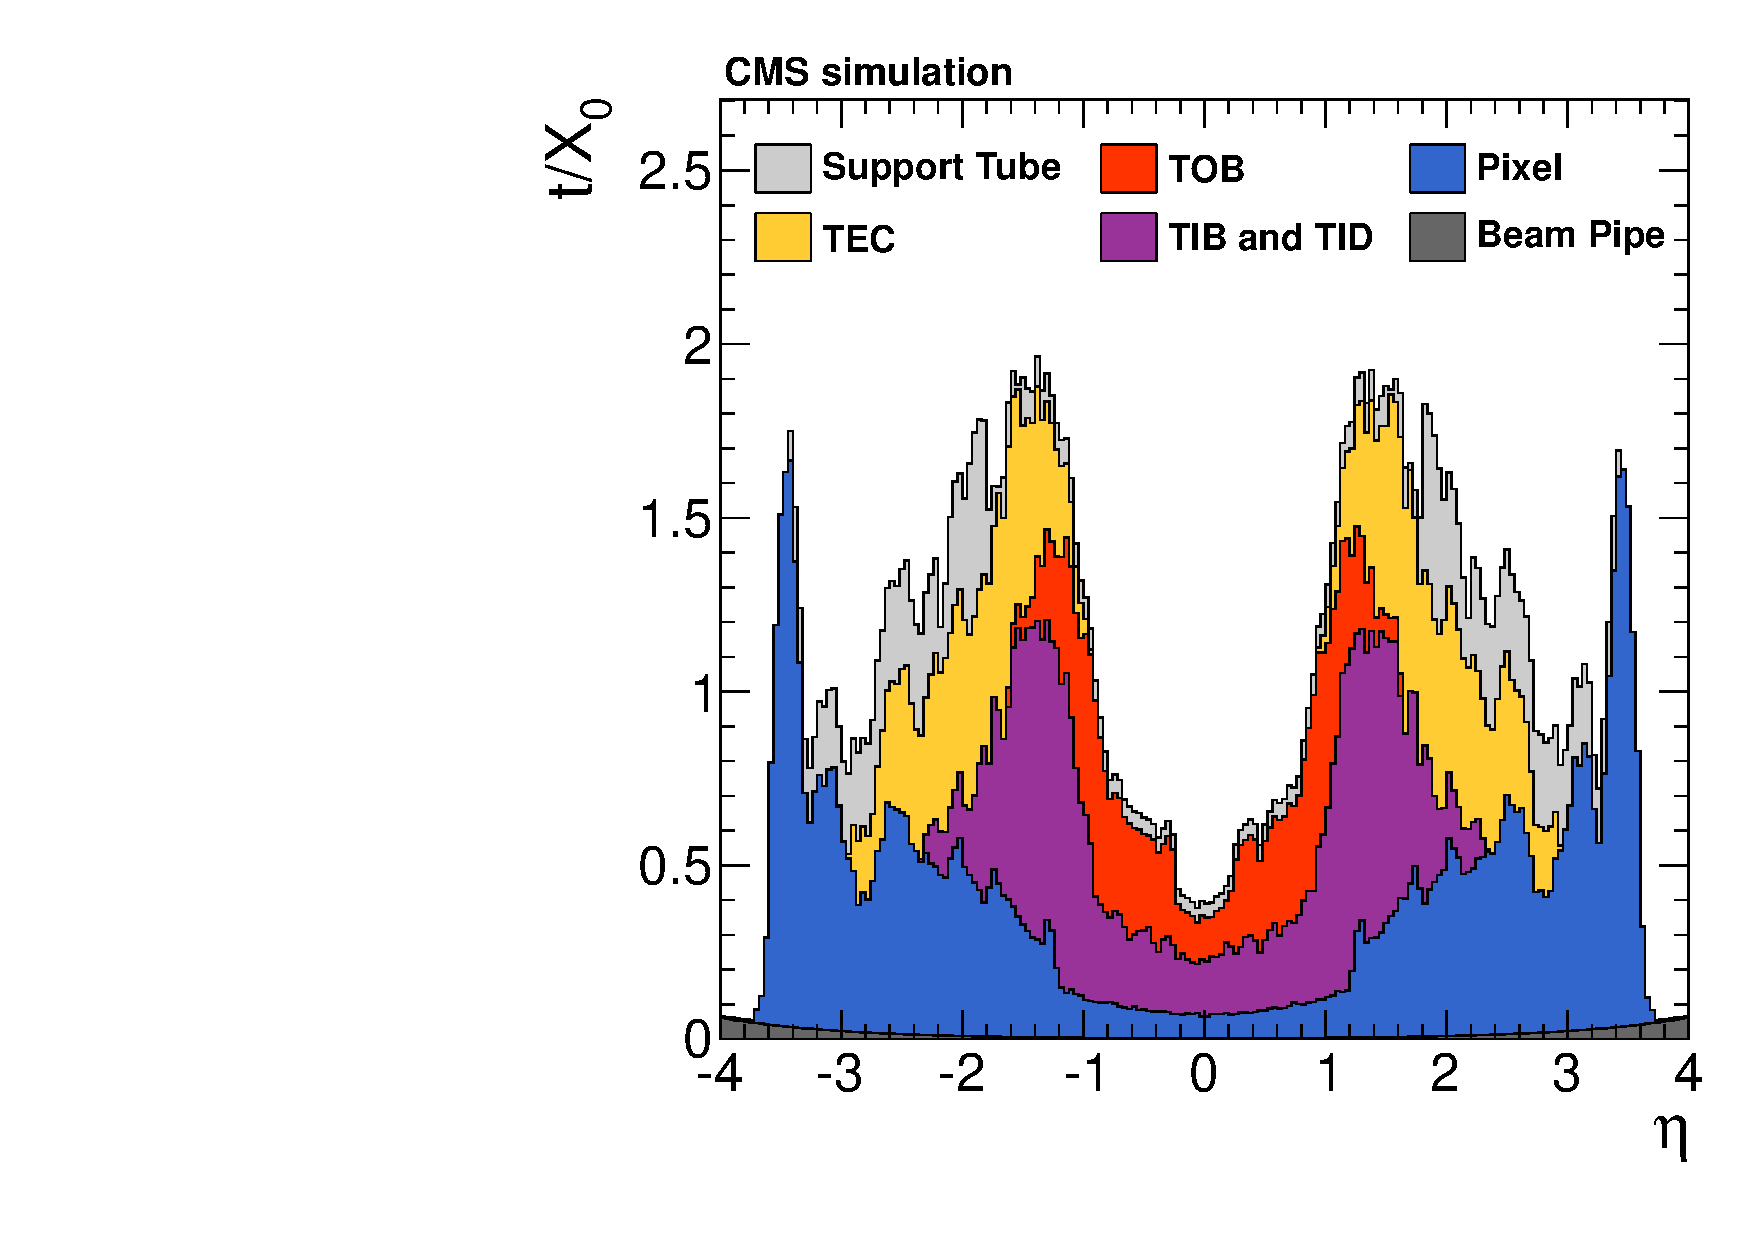
\includegraphics[width=0.4\textwidth]{figures/MaterialBudget_RadLengths.pdf}
    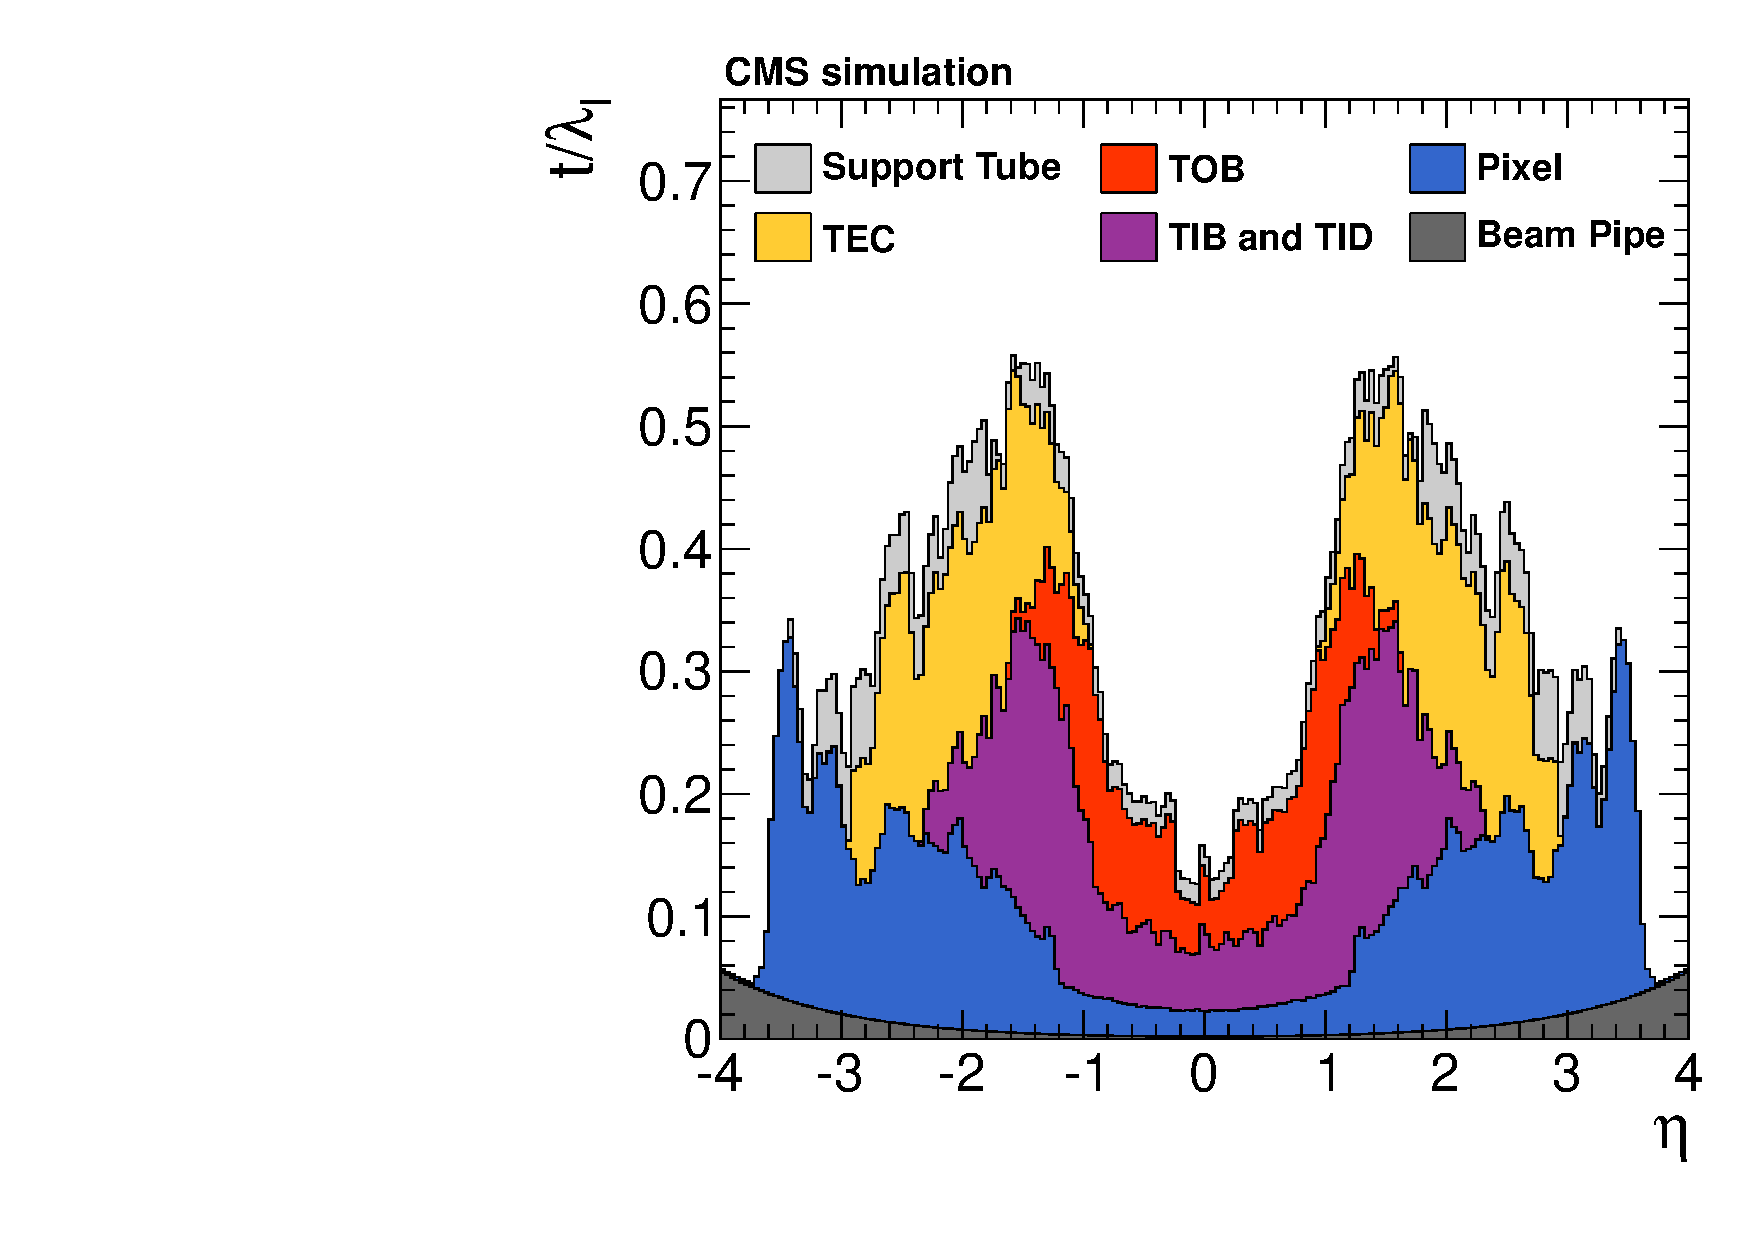
\includegraphics[width=0.4\textwidth]{figures/MaterialBudget_InteractionLengths.pdf}
    \caption[Tracker material budget.]{
      The CMS tracker material budget in (left) radiation lengths (ie electromagnetic) and (right) interaction lengths (ie nuclear), in the configuration used in 2016 and earlier. 
      While the CMS tracker is not intended to shower particles, only to measure positions as gently as possible, some amount of interaction between tracker material and collision products is inevitable.
      Taken from \cite{cmstracking}.}
    \label{fig:trackerbudget}
  \end{figure}  

  \begin{figure}[h!]
    \centering
    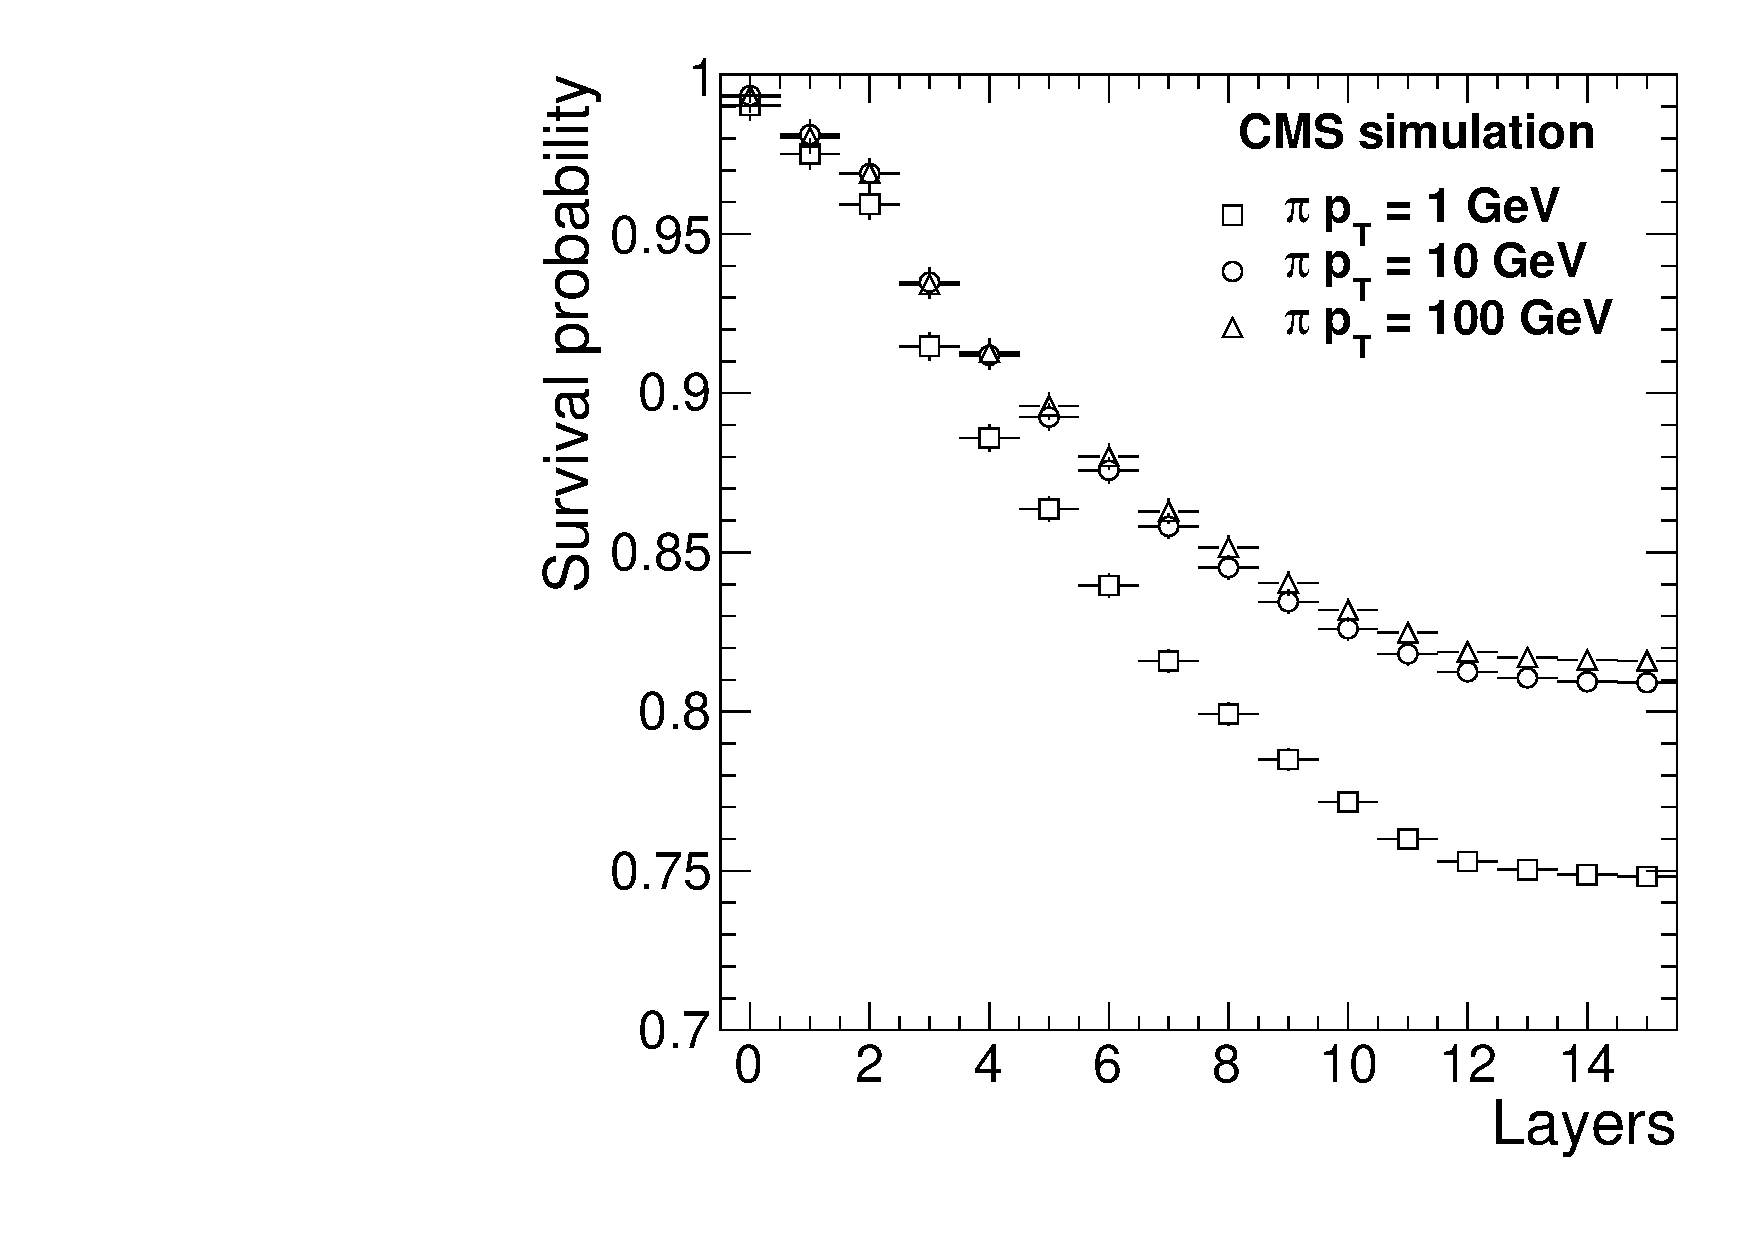
\includegraphics[width=0.85\textwidth]{figures/PionSurvivalProbability.pdf}
    \caption[Pion survival in the tracker.]{
      The probability for pions to undergo nuclear interactions in the CMS tracker by layer, in the configuration used in 2016 and earlier. 
      In rare cases, the pion may shower in such a way that no charged daughters have high enough energy to be reconstructed, causing its track to disappear.
      Taken from \cite{cmstracking}.}
    \label{fig:pionsurvival}
  \end{figure}  

  As a general rule, the tracker intends to interact with particles only to the extent absolutely necessary to measure their positions.
  Strong interactions between the tracker and the particles it is measuring modify the particles' tracks and affect their energies, and are therefore undesirable.
  Unfortunately, electrons are so strongly affected by bremsstrahlung that the tracker is quite thick in terms of radiation lengths, as shown in Figure~\ref{fig:trackerbudget} (left).
  Therefore, electrons at CMS are experimentally observed more as clouds of bremsstrahlung photons by the time they reach the electromagnetic calorimeter at CMS, and must be reconstructed with a special tracking procedure, the Gaussian-sum filter described in \cite{gsftracking}.
  In terms of interaction lengths, the CMS tracker is much thinner, as shown in Figure~\ref{fig:trackerbudget} (right).
  The vast majority of hadrons therefore reach the calorimeters without having undergone a nuclear interaction.
  Figure~\ref{fig:pionsurvival} shows that over 80\% of high energy charged pions reach the calorimeters intact.
  Even so, 80\% is not 100\%.
  Pion tracks occasionally terminate in a shower induced by a collision with a nucleus inside the tracker.
  In rare cases, these showers can contain {\it zero} visible particles of any kind.
  These disappearing pions constitute an important background for the disappearing tracks search.

  \subsection{Electromagnetic Calorimeter} \label{sec:ecal}

  The primary purpose of the electromagnetic calorimeter (ECAL) is to observe the energies of photons, which do not leave tracks.
  It is also important in the observation of electrons, which produce a jet of photons due to bremsstrahlung in the tracker.
  Other electromagnetically interacting particles will also leave small ECAL deposits, but much less due to their lesser tendency to produce photons.
  In Figure~\ref{fig:cmsreconstruction}, the electron (red) and photon (dotted blue) produce strong showers in the ECAL (green), while the other particles leave negligible deposits.

  The design prioritizes good resolution of photon energies and positions over all else, due to the experimental importance of the Higgs boson's decay to a pair of isolated photons.
  To accomplish this, the ECAL is constructed from tens of thousands of scintillating lead tungstate crystals, which has several desirable properties.

  First, these crystals have a Moliere radius of only 2.2~cm \cite{cms_tdr}.
  Aside from providing generally good position resolution, this small Moliere radius most importantly allows a prompt isolated photon, perhaps from a Higgs decay, to be distinguished from two closely overlapping photons produced by the decay of a neutral pion, because the two separate showers produced by the photon pair are clearly separated in the ECAL cells.
  These two nearby showers may merge into a single large shower indistinguishable from that of a single photon in a material with a larger Moliere radius.
  Similarly, photons produced inside jets can be distinguished from truly isolated photons, since the showers of other particles in the jets can be discriminated from the photon's own shower.
  Although the size of the shower is restricted, a typical one will still extend over a few adjacent crystals as shown in Figure~\ref{fig:cmsreconstruction}, so that a 5-by-5 cluster of crystals, or potentially a smeared supercluster for electrons that have radiated over a larger area, is the essential object of ECAL reconstruction.
  Studying the distribution of energy measurements across the crystals in a cluster, as described in \cite{ecal_algorithm}, allows for better fake rejection and energy resolution of 1\% \cite{ecal_energy_resolution}.

  Second, lead tungstate also has an extremely short radiation length, only 0.89~cm compared to the roughly 2 radiation lengths of the entire 1~m radius tracker, so it contains electrons very efficiently \cite{cms_tdr}.

  Third, scintillation in lead tungstate happens quickly, with 80\% of the light produced within 25~ns \cite{cms_tdr}. 
  This speed is critical for coping with the 25~ns bunch spacing of the LHC's proton beams, so that the ECAL deposits produced by adjacent bunch crossings can be distinguished.
  Due to this rapid shower production and careful calibration of the electronics, the ECAL achieves a timing resolution of roughly 0.2~ns for particles with momenta on the order of tens of GeV \cite{ecaltiming}.

  Finally, lead tungstate is resistant to radiation damage, so that the ECAL can continuously operate in the high flux environment of LHC proton collisions.
  Unfortunately, it is not immune to radiation damage, and so the performance of the ECAL degrades over time.
  By the end of data taking in 2018, roughly 20\% of ECAL cells no longer consistently detected showers of photons and electrons.
  This leads to a background for the disappearing tracks search consisting of electrons that transform to photons inside the tracker, no longer leaving a track, but are not later detected as photons in the ECAL.
  Fortunately, 80\% of the ECAL is still performing well despites years of high radiation flux, so this background can be almost entirely rejected by mapping and vetoing the poorly performing cells, using events in which a Z boson decayed to a pair of electrons, exactly one of which is lost due to this effect, as described in Section~\ref{sec:distracks}.

  \subsection{Hadronic Calorimeter} \label{sec:hcal}

  Charged hadrons are too massive to shower significantly in the ECAL, and neutral hadrons are invisible even to the tracker.
  However, both can be made to shower by capitalizing on their powerful nuclear interactions, and the hadronic calorimeter (HCAL) accomplishes this, as depicted in Figure~\ref{fig:cmsreconstruction} for a neutral hadron in dotted green and a charged hadron in solid green.
  The performance of the HCAL is very important to analyses selecting events containing jets and missing energy, as HCAL measurement errors lead directly to errors in jet energies, which in turn cause errors in the inferred missing energy in the event.

  The essential plan of the CMS HCAL design is to induce hadron showers by putting a high density of atomic nuclei in their paths in the form of 5~cm brass plates, then to measure the products of these showers using plastic scintillators, and from this reconstruct the energies of the original hadrons.
  To ensure that as few hadrons as feasible escape detection, whether from the primary interaction or from secondary showers, there are multiple layers of this shower-inducing metal plate and scintillator combination.
  Nevertheless, some hadrons do manage to ``punch through'' the HCAL, especially if they have extremely high energy, and even successful measurements are only accurate to within roughly a factor of 2 \cite{HCALphase1}, unless that hadron has very high energy.
  On the whole, the CMS HCAL performance is the weakest of any detector system.
  However, the energy of a typical jet is not measured only with the HCAL, and errors made on different hadrons within a jet tend to cancel, so that CMS achieves a typical jet energy resolution of approximately 10\%, for the jets of most interest \cite{cms_tdr}.
  Still, jets are occasionally badly mismeasured, most often due to HCAL measurement errors, and it is important for analyses selecting events with large missing energy to filter out these mismeasurement events, see Section~\ref{sec:MT2bg}.

  Accuracy of energy measurements aside, the ability to detect neutral hadrons consistently in the HCAL is important to the disappearing tracks search discussed in Section~\ref{sec:distracks}.
  A charged hadron can decay to a neutral hadron inside the tracker, and thus allow known Standard Model physics to produce an apparent disappearing track.
  Unlike a true disappearing track, however, the neutral hadron is detectable in the HCAL, revealing what happened in the tracker and rejecting this Standard Model background.
  As with the ECAL, poorly performing regions of the HCAL can be vetoed to ensure this background is wholly rejected.

  \subsection{Muon System} \label{sec:muon}

  The muon system is the outermost detector of CMS, and the only one outside the solenoid.
  Muons, like charged hadrons, are too heavy to produce significant showers in the ECAL, and unlike hadrons, do not have nuclear interactions allowing them to be trapped in the HCAL.
  Instead, they penetrate through the entire detector, leaving a track in the tracker, largely disappearing inside the calorimeters, and then reappearing in the muon system.
  Unlike other particles, then, the energies of muons must be measured largely by analyzing the curvature of their tracks.
  As one of the design goals of the Compact Muon Solenoid experiment is ultra-precise measurements of muons, the muon system is large partly in order to provide a long look at the muon's track for momentum measurement purposes, and partly to provide a positive identification of a particle as a muon, rather than a hadron that managed to escape the HCAL, as only muons can penetrate through so many layers of detector material.
  As installing a second tracker would be far too expensive and excessive, the muon system instead uses only four widely spaced layers of detectors operating based on ionization of gas by passing muons, which while generally worse than the tracker system in terms of space and time resolution, are much more economical for covering such a large volume \cite{cms_tdr}.
  The design of CMS has proven successful. 
  Muons are by far the cleanest, most well-measured particles at CMS, with momentum resolution better than 1\% and high efficiency, as we have already seen for tracker muon tracks in Figure~\ref{trackefficiency}.

  While muons are the only charged Standard Model particle that can consistently penetrate to the muon system, the possibility exists that heavy long-lived charged particles beyond the Standard Model may be produced in LHC collisions and leave hits in the muon system.
  The disappearing tracks search in Section~\ref{sec:distracks} targets models that could potentially produce such a signature.
  However, that search considers only tracks that disappear inside the tracker, and in fact explicitly vetoes muon-like tracks, so it is not sensitive to this potential signature.
  Adding sensitivity to this powerful signature could be an interesting extension in the future.

  \subsection{Missing Transverse Energy} \label{sec:MET}

  Once muons are measured in the muon system, all Standard Model particles have been accounted for, except neutrinos.
  Unfortunately, the neutrino interaction length, even at LHC energies, is on the order of billions of meters at Earthly densities, so that the probability of a typical LHC neutrino experiencing even a single interaction anywhere inside the CMS detector is negligible \cite{neutrinos}.
  However, the presence of neutrinos can be inferred by measuring all other particles inside the event, and observing that the transverse momentum does not balance, indicating either the presence of at least one undetected particle, or a detector mismeasurement.
  At a hadron collider like the LHC, only the transverse momentum can be used for this procedure, because the exact center of momentum frame of the primary collision is unknown along the beam axis.
  The actual colliding particles are not the protons themselves, but rather subcomponents of the proton called partons.
  The partons are approximately at rest with respect to the detector in the transverse plane, so that their transverse momenta are known to sum nearly to zero, but have unkonwn momenta along the beam axis.
  Unbalanced momentum along this axis may indicate the presence of an invisible particle, but more often it indicates simply that the initial momentum of the collision along the beam axis was nonzero.
  The observable is not the missing energy, then, but the missing transverse energy, written as MET or \met.
  This observable is tentatively identified with the unobservable transverse momentum of a neutrino.

  Although the invisible momentum is only available in the transverse plane, it is still a very useful quantity.
  For instance, consider the leptonic decay of a W boson, $W^{\pm}\rightarrow\ell^{\pm}\nu$.
  The W boson has mass approximately 80~GeV with width approximately 2 GeV \cite{pdg}.
  Even allowing for detector resolution effects around 10\%, a lepton and neutrino system originating from an on-shell W decay can never have mass greater than approximately 100~GeV.
  It follows directly that transverse mass \Mt, the mass calculated using energy and momentum in the transverse plane, also cannot exceed 100~GeV, since $E_T < E$ and $\pt < p$.
  The analyses discussed in the next Section~\ref{sec:analysis} leverage this fact to determine whether a lepton or disappearing track may potentially have originated in a leptonic W decay.
  
  Of course, while the missing transverse energy is sometimes the undetected energy of a single neutrino or unknown invisible particle, it can also be a consequence of mismeasurement, or even potentially the vector sum of the transverse momenta of {\it multiple} undetected particles.
  In fact, even events with relatively large amounts of missing energy at CMS are most often produced by detector mismeasurement (see Figure~\ref{fig:mt2dist}, in which ``Multijet'' events in yellow have \met due to detector mismeasurement), even though such large errors are rare, because neutrinos are rarer still.
  Searches for invisible particles naturally wish to eliminate these events with fake \met using cleaning selections.
  One of the most powerful observables that can be used to reject events with fake \met is \mttwo \cite{mt2}, a generalization of \Mt.

    \subsubsection{\mttwo} \label{sec:MT2}

    Although the presence of invisible particles can be inferred via the observation of a nonzero \met vector, it is not trivial to distinguish events in which the \met corresponds to the transverse momentum of a single invisible particle, and events in which the \met is the vector sum of the momenta of multiple invisible particles.
    It can also be difficult to distinguish the presence of genuine invisible particles from cases of detector mismeasurement.
    While no conclusions about invisible content can ever be drawn with perfect certainty for any single event, the situation is not hopeless.
    The \mttwo observable is one tool used to make quantitative inferences concerning an event's invisible content.
    Specifically, \mttwo is designed to identify events consistent with the presence of two invisible particles in the final state, produced in symmetric decay chains of pair-produced heavy particles.
    This also tends to reject events in which the \met was produced by detector mismeasurement, as these events tend to have no symmetry whatsoever.

    The algorithm begins by dividing the visible portion of the event into two hemispheres.
    To do this, an event must have at least two visible objects, so in an event with only hadron jets, like the majority of the events at CMS, \mttwo can be calculated only for multijet events.
    The method used to assign each visible object to a hemisphere varies.
    One popular method, and the one used in \cite{MT2_2019}, begins by identifying the pair of objects with largest system mass, $M_{12}$,
    \begin{equation} \label{eqn:dijetmass}
      M_{12} = \sqrt{(E_1+E_2)^2-(\vec{p}_1+\vec{p}_2)^2},
    \end{equation}
    and assigning each as the seed of a separate hemisphere.
    In an event containing two identical pair-produced particles undergoing similar decay chains, the pair of objects with largest mass is unlikely to originate from the same particle, as the mass of the full system is strictly greater than the mass of either particle.

    Then, each object is associated to the seed of lesser Lund distance, $D_{L}$, which is defined for seed $i$ as \cite{lund1,lund2},
    \begin{equation} \label{eqn:lund}
      D_L = (E_{i}-p_{i}\cos\theta)\frac{E_{i}}{(E_{i}+E)^2}
    \end{equation}
    where $E_i$ is the seed's energy, $p_i$ is the seed's momentum, $\theta$ is the angle between the momenta of the seed and of the object under consideration, and $E$ is that object's energy.
    Considering the massless limit of $D_L$ provides some intuition,
    \begin{equation} \label{eqn:lund}
      D_L = \frac{1-\cos\theta}{(1+\frac{E}{E_h})^2}.
    \end{equation}
    The Lund distance is small if the hemisphere and object point in nearly the same direction so that $\cos\theta\sim1$, and if $E_i$ is small.
    Thus, selecting based on minimal Lund distance prefers to assign objects to the less energetic seed when possible to keep the hemispheres energetically balanced, so long as the object and the seed point in similar directions.
    Once all objects have been assigned to a seed, two new seeds are defined as the sum of all the four-momenta in each hemisphere, and the assignment procedure repeats using these seeds.
    This continues until no object changes hemisphere after an iteration.
    Ultimately, the algorithm assigns objects to the correct hemisphere with efficiency ranging from approximately 70--85\%, with higher efficiencies obtained in events with fewer objects and therefore reduced combinatorics \cite{lundeff}.

    The next step of the calculation of \mttwo takes these finalized hemispheres as inputs.
    Under the hypothesis that the observed missing energy is the vector sum of the unobserved momenta of two invisible particles, the algorithm considers every possible vector decomposition,
    \begin{equation}
      \ptvecmiss = \vec{v}_1+\vec{v}_2
    \end{equation}
    and calculates \Mt for hemisphere $i$ with respect to $\vec{v}_i$.
    The maximum of these two values of \Mt is taken as the {\it candidate} \mttwo for this decomposition.
    This choice is motivated by a desire to infer the true mass of the decaying pair-produced particle, again, under the hypothesis that there are two pair-produced particles undergoing symmetric partially invisible decays.
    For the correct \ptvecmiss decomposition and hemisphere assignments, the two calculated transverse masses are correct, and both are no larger than the true mass of the pair-produced particles. 
    The larger, of course, is nearer to that true mass.
    
    The only remaining step is to select which of the candidate values of \mttwo, equivalently which \ptvecmiss decomposition, is correct.
    The algorithm selects the smallest candidate \mttwo value found, the ``minimum maximum,'' so that the final \mttwo is
    \begin{equation} \label{eqn:minmax}
      \mttwo = \underset{\ptvecmiss = \vec{v}_1+\vec{v}_2}{\min}\left[\max\left(\Mt^1,\Mt^2\right)\right]
    \end{equation}
    where hemispheres 1 and 2 are assembled as described above.
    Since the correct missing energy decomposition is among those considered and manifestly cannot produce a value of \Mt greater than the true mass of the parent particle when hemisphere assignments are correct, selecting the ``minimum maximum'' guarantees that \mttwo can be no larger than the mass of the parent particle. 
    Just as \Mt cannot exceed the mass, \mttwo is unlikely to exceed the true \Mt.

    Of course, it is possible for \mttwo to be small even in genuine signal events for which it is designed to be large, and it is possible for especially pathological mismeasurement events to have large \mttwo despite \mttwo being a powerful rejector of these backgrounds (see Section~\ref{sec:MT2QCD}).
    No observable is so magical that it can accept 100\% of signal and reject 100\% of background.
    Still, \mttwo is one of the most powerful discriminants available for analyses targeting pair-produced particles decaying semi-invisibly, as can be seen for instance in Figure~\ref{fig:mt2dist}.
    Indeed, the selection of $\mttwo > 200$~GeV applied by the analyses discussed in Section~\ref{sec:analysis} is the single most important part of their baseline selection, dramatically reducing especially the detector mismeasurement background.

\section{CMS Event Reconstruction} \label{sec:reconstruction}

After observing the signatures of particles in the detector, CMS must reconstruct what happened in the event.
A fully detailed description is well beyond of this document and indeed, well beyond the scope of any single document.
This section will describe only some of the most essential pieces that have not already been covered by previous sections.

  \subsection{Pileup and the Trigger System} \label{sec:pileupandtrigger}

  Previous sections have discussed some of the challenges faced by the detector in reconstructing a single collision.
  However, the large event rate at CMS produces its own set of challenges.
  First, the sheer number of bunch crossings per second produces too high a data rate to save the measurements of all but a small subset of collisions \cite{cmstdr}.
  Second, the collision of protons in bunches rather than singly to maintain a high data produces multiple simultaneous collisions in each bunch crossing, called pileup, which must be disentangled.
  
    \subsubsection{The Trigger System} \label{sec:trigger}

    The LHC provides CMS with roughly 1 billion collisions per second spread across 40 million bunch crossings per second, one per 25~ns.
    This enormous event rate is necessary to provide sensitivity to very rare physics.
    For instance, the expected number of gluino pair-production events observed at CMS is approximately 1 across the entire 2016, 2017, and 2018 datasets, for a gluino mass of 3~TeV.
    Unfortunately, as each bunch crossing constitutes roughly 1.5~MB of data, it is feasible to write only approximately 100 events per second to disk, for 150~MB/s \cite{cmstdr}.
    All but one bunch crossing in 400,000 must be rejected, a feat accomplished by a two-tier trigger system \cite{trigger}.
    
    The Level-1 trigger system is implemented in hardware and considers gross features of the event that are rapidly computable and qualify it for further consideration.
    It rejects the vast majority of bunch crossings, reducing the rate from 40~MHz to 100~kHz.
    The rejected events are almost all mundane events containing only a few low energy hadron jets.
    Some of the signatures that may qualify an event for further consideration include measurements in the muon system consistent with an isolated muon of a minimum \pt, or preliminary signs that the event may have large missing energy.
    The Level-1 trigger system is allotted only 3.2~$\mu$s to make a decision, of which less than 1~$\mu$s is available to perform a limited reconstruction, and so is subject to errors that can cause it to incorrectly reject some borderline events, so that the trigger is not a perfect step function.
    For instance, the electron energy resolution of the Level-1 reconstruction is shown in Figure~\ref{fig:L1res} (upper), along with the resulting trigger turn-on curve (lower).
    To avoid the need to simulate this trigger turn on, analyses typically select only events sufficiently distinctive that they are accepted by the trigger with 100\% efficiency.

    \begin{figure}[h!]
      \centering
      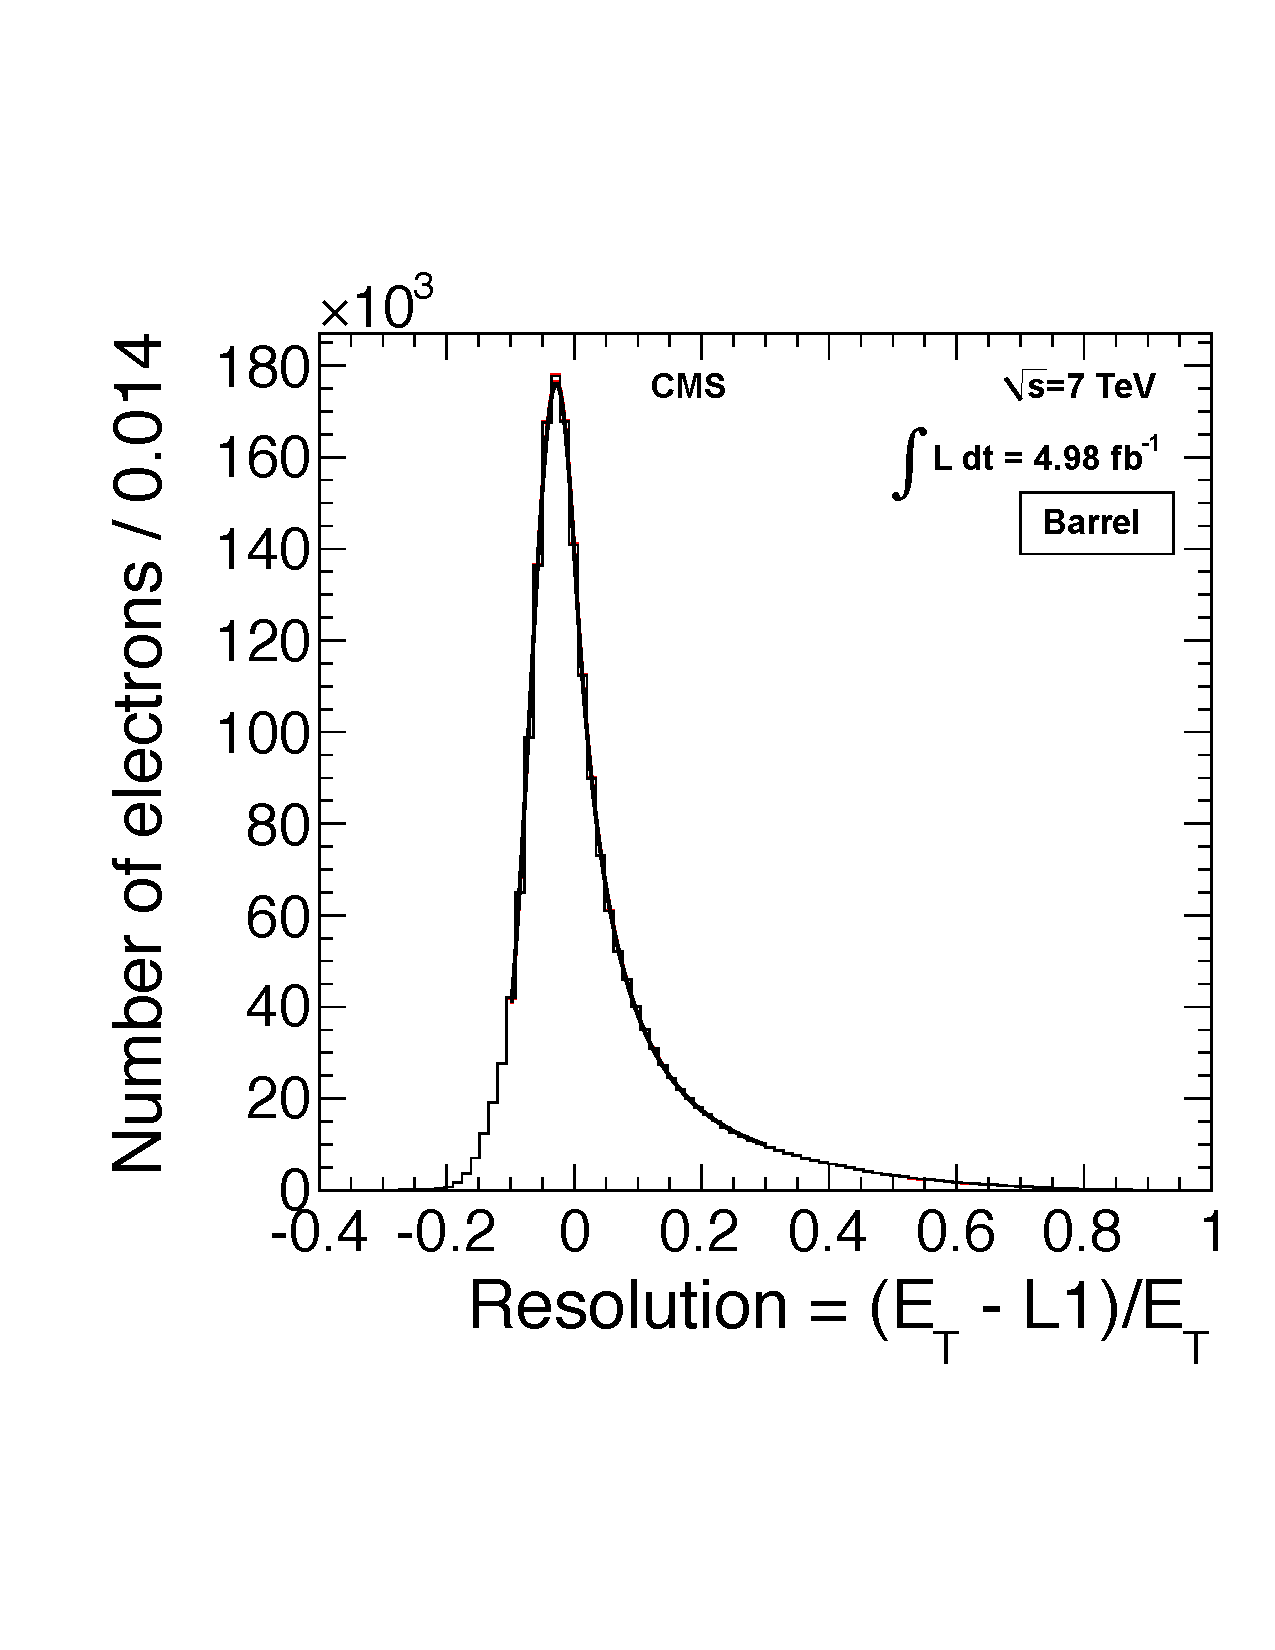
\includegraphics[width=0.55\textwidth]{figures/L1_res.pdf}\\
      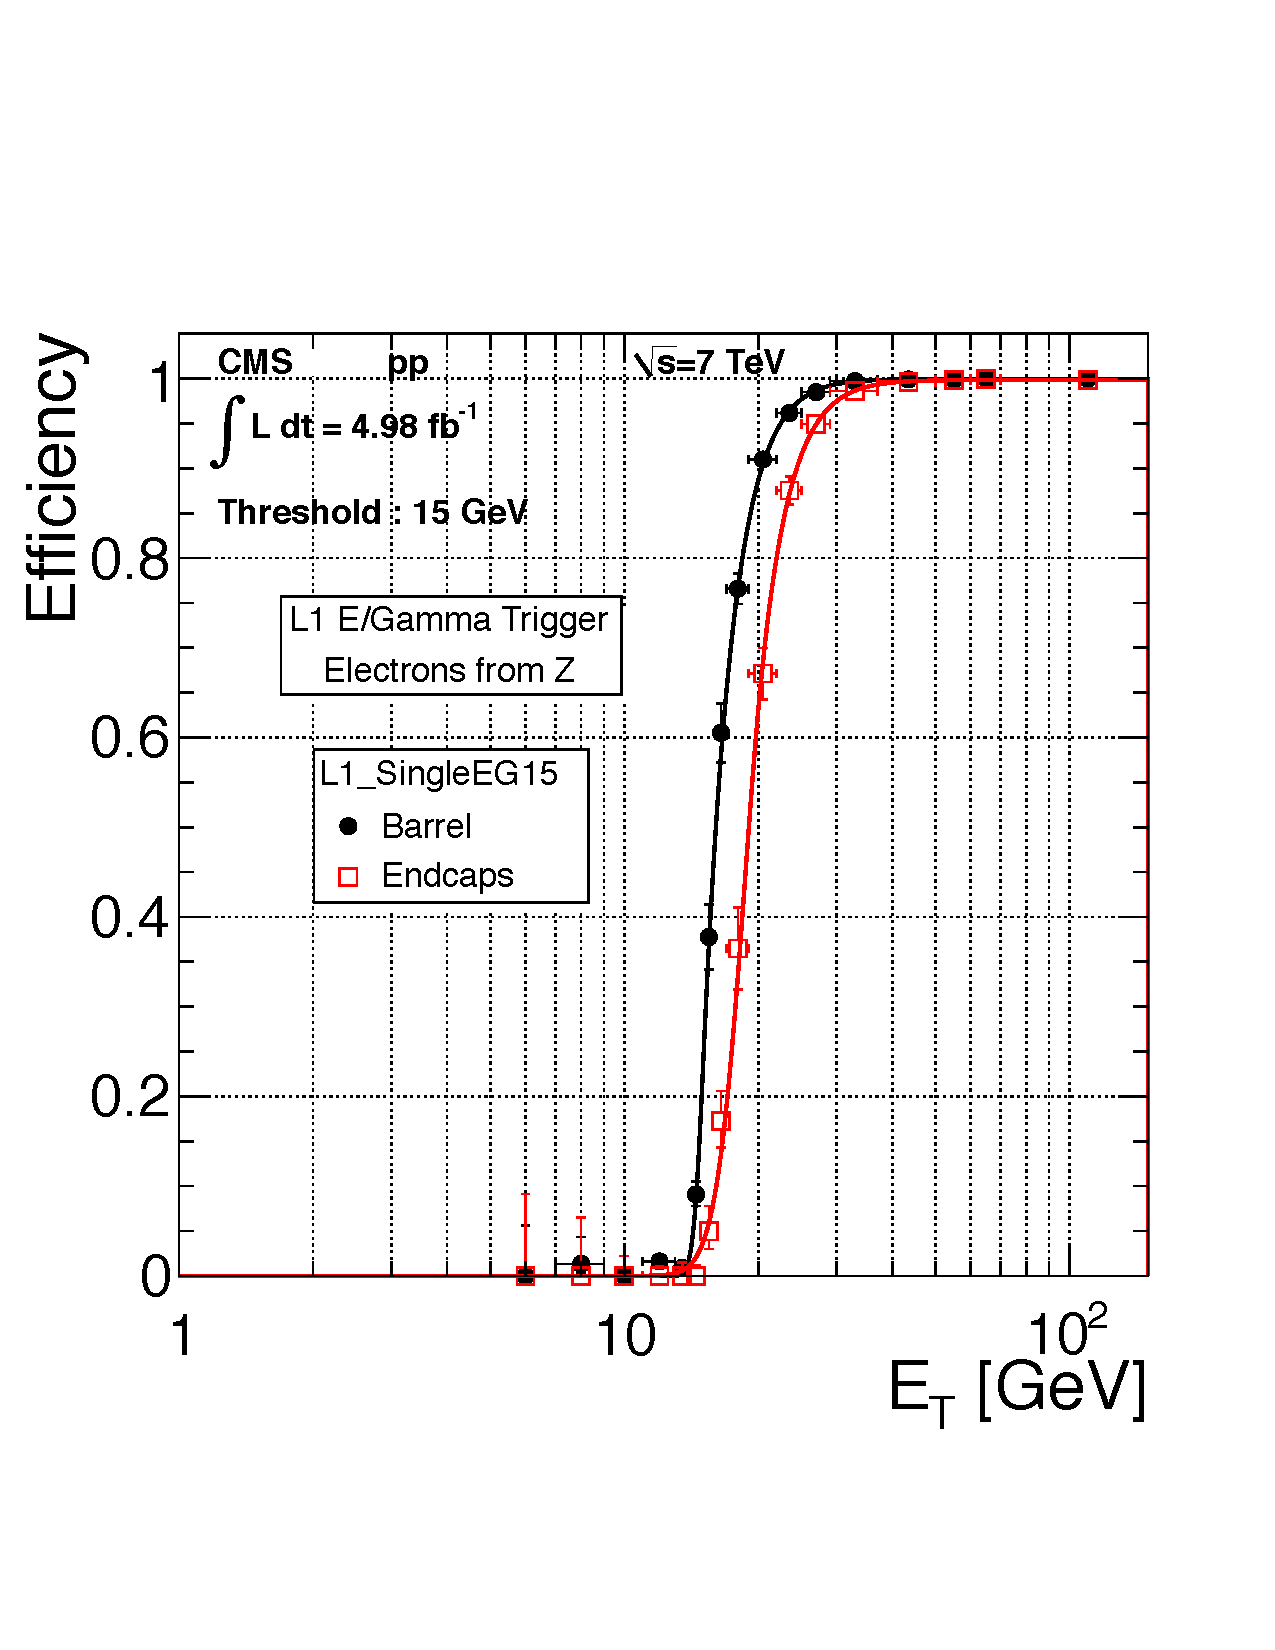
\includegraphics[width=0.55\textwidth]{figures/electron_turnon.pdf}
      \caption[Level-1 trigger electron energy resolution and associated turn-on curve.]{
        (Upper) The electron energy resolution of the Level-1 CMS trigger obtained in 7~TeV collisions, in the barrel.
        Positive values correspond to incorrectly small measurements of the electron energy, and may cause candidate electrons to fall short of the minimum energy requirement, leading to a trigger inefficiency.
        (Lower) The Level-1 electron trigger turn-on curve as a function of offline reconstructed electron energy, with a nominal threshold of 15~GeV.
        The black markers are for electrons in the barrel, corresponding to the electron population whose energy resolution is shown in the upper plot, and red is for electrons in the endcaps.
        To avoid exposing itself to trigger turn-on systematic uncertainties, an analysis may be forced to select only events possessing an electron with energy greater than 30~GeV, despite the trigger nominally accepting events containing an electron with energy as low as 15~GeV.
        Taken from \cite{trigger}.}
      \label{fig:L1res}
    \end{figure}      

    Events passing the Level-1 trigger are subjected to a more careful analysis by the High Level trigger (HLT), implemented in software on standard servers.
    With 13,000 machines working in parallel, the HLT is allotted 90~ms per event, enough time for reconstruction of the portion of the event identified by the Level-1 trigger as interesting at near offline quality.
    One event in 1000 considered by the HLT is sufficiently spectacular to qualify to be written to disk, and these constitute the CMS dataset available for final offline analysis.

    \subsubsection{Pileup Correction} \label{sec:pileup}

    Obtaining a high enough event leads to many simultaneous collisions (not 1 proton collision at a time, but bunches crossing every 25 ns).
    Charged pileup contribution can be subtracted exactly using the tracker, but neutral pileup correction is heuristic.
    Effective area vs delta-beta.

    In addition to the high bunch crossing rate, the reconstruction also must cope with the large number of simultenous collisions in each bunch crossing, called pileup.
    The mean number of pileup collisions was 32 in 2018 \cite{lumipublic}, and a significant number of bunch crossings exceeded 60 pileup collisions, as can be seen in Figure~\ref{fig:pileup}.
    Given that only one bunch crossing in 400,000 contains a collision interesting enough to be written to disk, the number of interesting collisions per bunch crossing is at most 1, and the others must be subtracted.

    \begin{figure}[h!]
      \centering
      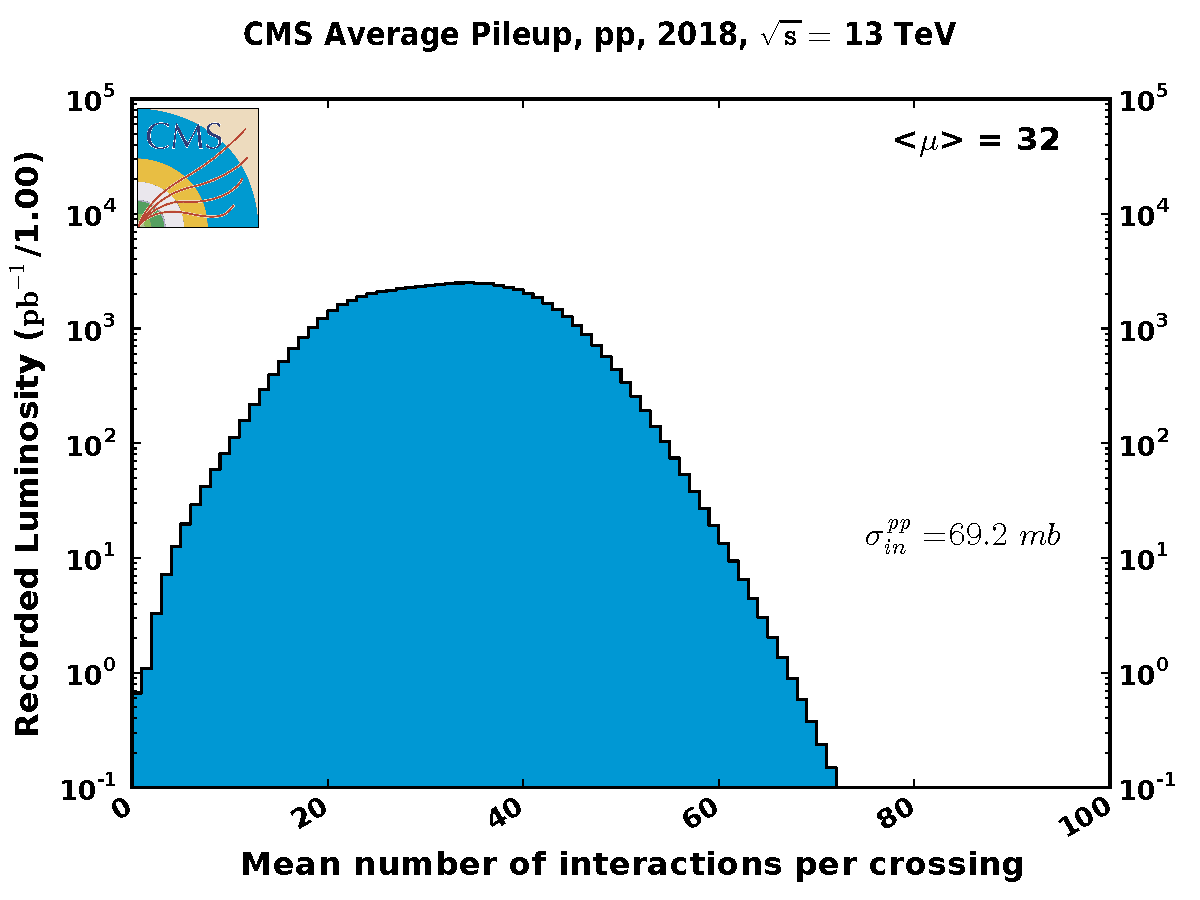
\includegraphics[width=0.65\textwidth]{figures/pileup.pdf}
      \caption[Pileup distribution in 2018.]{
        The distribution in 2018 of the number of simultaneous collisions per bunch crossing, so-called pileup, provided by the LHC and observed by CMS.
        The average bunch crossing produced 32 simultaneous collisions, with an inferred total inelastic collision cross section of 69.2~mb.
        Taken from \cite{lumipublic}.}
      \label{fig:pileup}
    \end{figure}  

    Barring errors in track reconstruction, charged pileup can be subtracted perfectly \cite{pileup}.
    Charged particles produce tracks, which can be associated to vertices.
    Tracks associated to vertices other than the primary vertex of interest can be subtracted.
    This is not possible for the neutral content of an event, which is known only from calorimeter deposits.
    
    There exist two popular heuristic methods for subtracting neutral pileup.
    The first method, called Delta-Beta, proposes that the neutral energy from a pileup vertex is equal everywhere to exactly one half of the charged pileup, because particles with charges +1, -1, or 0 tend to be produced with roughly equal probability and energy.
    This is true on average, but of course is only approximately true in any given instance.
    The second method, called Effective Area, benefits from larger pileup and has gained popularity recently.
    This method divides the detector into many small regions and calculates the median energy density in these regions, $\rho$.
    By taking the median, the calculation naturally mitigates the impact of outlier regions of the detector with large contributions from the primary vertex, which tends to be much more energetic than any of the pileup vertices.
    This median energy deposit is taken to be representative of the pileup contribution in every region of the detector, true by construction within statistical fluctuations, and subtracted everywhere to leave only the energy believed to originate from the primary vertex.
    This algorithm is only as accurate as the statistical fluctuations of pileup energy are small, and so benefits directly from increased pileup vertex counts.
    At present, both algorithms have similar performance and see wide use.
    The search in Section~\ref{sec:MT2classic} uses Effective Area, while the extension to this search in Section~\ref{sec:distracks} uses the Delta-Beta method to correct the isolation of disappearing tracks similarly.

    Pileup also makes reconstruction more difficult in a more general sense by overwhelming reconstruction algorithms.
    Of special importance to the Section~\ref{sec:distracks} disappearing tracks analysis is its effect on track fake rates.
    High pileup vertex counts cause proportionally increased hit counts in the tracker.
    With more hits to consider, the track reconstruction algorithm is more prone to make errors, and connect hits to form tracks that are not all associated with the same genuine particle.
    For instance, the algorithm may output a fake track using three hits produced by particles from three different pileup vertices that happen to fall in a line extrapolating to the primary vertex.
    The tracker is also overwhelmed at the hardware level, with higher particle flux causing higher operating temperatures, and therefore more noise, and overflowing readout buffers during periods where the beam luminosity, and therefore the typical pileup, is especially high \cite{cms_tracker}, as shown in Figure~\ref{fig:hitefflumi}.
    Events containing disappearing tracks, especially very short tracks, disproportionately originate from events at the extreme high end of the pileup distribution, indicating that pileup and, more generally, high beam luminosity directly causes background for this search by inducing track reconstruction errors.

    \begin{figure}[h!]
      \centering
      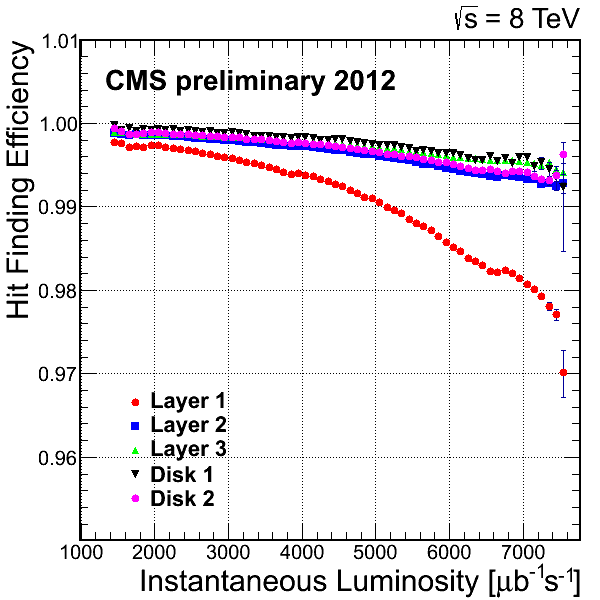
\includegraphics[width=0.65\textwidth]{figures/HitEff_vs_InstLumi.png}
      \caption[Hit efficiency as a function of instantaneous beam luminosity.]{
        The efficiency for a charged particle to leave a hit drops at high instantaneous beam luminosity, especially in the first layer of the tracker (red).
        Periods of high luminosity tend to produce events with high pileup.
        Taken from \cite{cms_tracker}.}
      \label{fig:hitefflumi}
    \end{figure}  

  \subsection{Particle Flow} \label{sec:particleflow}

  The general purpose offline reconstruction algorithm used in most cases at CMS is called Particle Flow \cite{particleflow}.
  Particle Flow (PF) attempts to reconstruct every individual particle in an event by integrating information from all detector components, producing so-called PF candidates.
  Rather than, say, obtain an energy measurement entirely from the calorimeters and ignore the energy measurement that can be made using the curvature of a particle's track, PF uses the tracker and the calorimeters as checks on each other, and intelligently assigns a final energy based on its beliefs about the relative trustworthiness of each measurement in each case.
  This extraction of all available information from the event rather than the traditional segregated inputs from different detector components is in part responsible for CMS's tremendous successes in pursuits like b-tagging, which achieves especially high efficiency by considering all possible clues simultaneously using a machine learning approach, rather than for instance using only the secondary vertex and track multiplicity information provided by the tracker \cite{particleflow}, or electron identification efficiency, as shown in Figure~\ref{fig:PFimprovement}.
  
    \begin{figure}[h!]
      \centering
      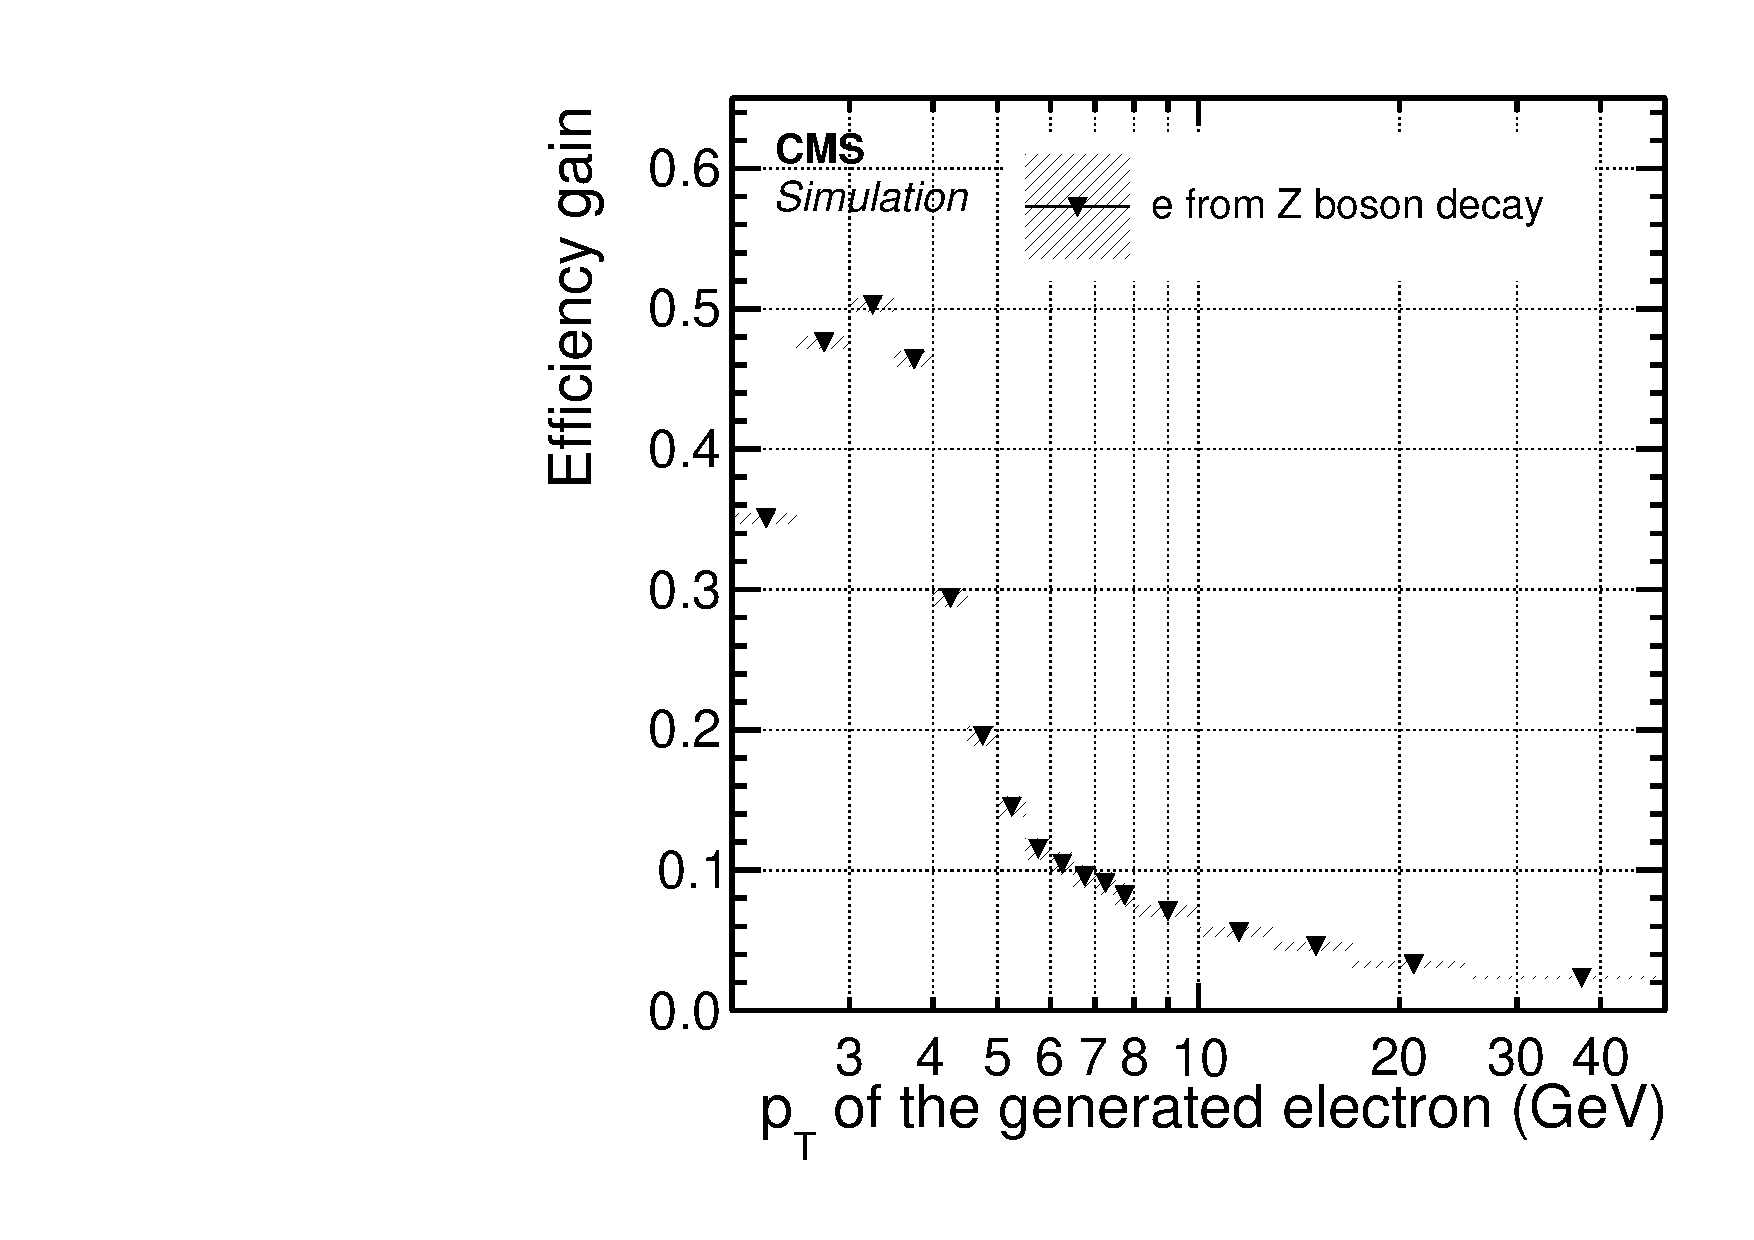
\includegraphics[width=0.65\textwidth]{figures/pfimprovement.pdf}
      \caption[Improvement of electron identification efficiency as a function of \pt using an integrated reconstruction approach like Particle Flow.]{
        The identification efficiency of electrons produced by the decay of a Z boson is dramatically improved by using information from both the tracker and the ECAL, rather than the ECAL alone as has been the standard approach in other detectors at hadron colliders.
        The absolute efficiency gain, $\mathrm{Eff}_{\mathrm{ECAL}+\mathrm{Tracker}}-\mathrm{Eff}_{\mathrm{ECAL}}$ is plotted.
        Taken from \cite{particleflow}.}
      \label{fig:PFimprovement}
    \end{figure}  


  This approach can allow PF to reject fakes or badly mismeasured particles.
  For instance, PF rejects tracks that do not extrapolate to significant calorimeter desposits, indicating that they are neither electrons nor hadrons, and also do not have a corresponding track in the muon chamber.
  In most cases, PF is correct to reject these tracks, which are almost assuredly fakes.
  In rare cases, the track is of such high quality that it passes the ``high purity'' selection described in Section~\ref{sec:tracker}, indicating that the tracker is highly unlikely to have made an error.
  These are called ``Lost Tracks,'' and are the foundational object for the track selection used in the Section~\ref{sec:distracks} disappearing tracks analysis.
  The fact that PF rejected these tracks despite a strong tracker measurement flags them as worthy of further study, serving as a useful clue for searches for new physics.
  
  \subsection{Jet Clustering} \label{sec:jetclustering}

  Jets produced by hadron fragmentation are constructed from PF candidates using the Anti-$k_t$ algorithm \cite{antikt}.
  A major goal of such an algorithm is including all of the content associated with a hadron's fragmentation in a single jet, and nothing else.
  Additionally, it is desirable for jets output by an algorithm not to be affected by very low energy particles that may be simple manifestations of noise, so that the same event measured by multiple detectors with different properties would produce nearly identical jets in every case.
  Older jet clustering algorithms simply used a fixed cone size, and included in jets anything that fell inside a cone centered on a few of the larger energy deposits in the calorimeters.
  Modern algorithms start at the particle level and associate particles to jets using distance measures similar to the Lund distance (Equation~\ref{eqn:lund}) used in \mttwo.
  The Anti-$k_t$ algorithm uses the measure of distance between particles $i$ and $j$ defined as
  \begin{equation} \label{eqn:antikt}
    d_{ij} = \min\left(\frac{1}{k_{ti}^2},\frac{1}{k_{tj}^2}\right)\frac{\Delta R_{ij}^2}{R^2}
  \end{equation}
  where $\Delta R_{ij}^2=(\eta_i-\eta_j)^2 + (\phi_i-\phi_j)^2$, $R$ is a tunable jet cone size parameter, and $k_{ti}$ is the \pt of particle $i$.
  The algorithm gets its name from the appearance of $k_t^2$ in the denominator rather than the numerator of the minimum as in its predecessor, the $k_t$ algorithm.
  The most important advantage of this algorithm relative to its predecessor is the suppression of the effect of very low energy particles on jet composition and shape by using the minimum of $1/k_t$ rather than of $k_t$.
  This causes low energy particles to cluster not simply with whatever the nearest particles are, but rather with the nearest {\it high energy} particle, since $d_ij$ is always large for two low energy particles, while it is suppressed by the smallness of the high energy particle's $1/k_t^2$ in any pairing with a low energy particle.
  Nearby hadrons producing partially overlapping jets can thereby be distinguished, by clustering the lower energy particles around nearby but separate high energy cores, instead of forming one fat jet from the agglomeration of all particles falling inside the cone, and jets can pick up low energy particles that may have been radiated a moderate distance away from the core of the source jet, instead of these outliers clustering amongst themselves to form spurious jets.
  Thus, jets clustered by the modern Anti-$k_t$ algorithm closely correspond to the source hadrons, making the \njet observable more useful than ever before, and also assisting flavor tagging.

\section{Simulation} \label{sec:simulation}

  The Standard Model and hypothetical models of new physics predict what happens at the primary interaction.
  These parton-level predictions need to be converted into final state particles, and then a prediction of the observable signatures produced by these particles in the detector.
  To accomplish this, CMS employs a multi-tier Monte Carlo simulation process.

  \section{Objectives} \label{sec:objectives}

  Simulation is used both to understand sources of background and to predict the appearance and yield of signals.
  Although simulation is subject to uncertainties that cause analyses to prefer using data driven backgrounds, it still captures the gross features of all but the most pathological background sources.
  For understanding the expected appearance of signals, it is the only option available.

  \section{Limitations and Challenges} \label{sec:limitations}

  Simulation of collider physics faces four primary challenges.

  First and foremost is a finite computation budget. 
  All simulations must be performed numerically, using a Monte Carlo approach.
  While the physical collider can produce 1 billion event per second and thereby produce events with extremely rare properties, such an event rate is orders of magnitude out of reach of software.
  This is not necessarily a problem for rare signal models, as a computer can be made to simulate only the signal model of interest, and ignore the much more common background physics, producing simulated events even faster than the collider would produce.
  However, much more common backgrounds are typically difficult to simulate in the phase space of greatest interest.
  For instance, QCD events with large \mttwo are extremely rare as discussed in Section~\ref{sec:MT2bg}, but QCD events comprise nearly all of the 1 billion collisions per second observed at CMS, such that even the high \mttwo event rate is non-negligible.
  Software simply cannot produce a statistically robust sample of these events using the traditional Monte Carlo sampling approach.
  Section~\ref{sec:RandS} discusses a successful workaround for this problem.

  The other three problems affect three separate stages of the simulation pipeline.

  First is an uncertainty arising from theory due to the perturbative approximation used to extract predictions from the Standard Model at parton level.
  Although the Standard Model is capable of producing astonishingly accurate predictions, famously including over 10 digits of accuracy in its prediction of the electron's magnetic moment \cite{electronmu_exp}, calculating predictions to such precision is a laborious undertaking that cannot practically be managed for every conceivable process \cite{electronmu_th}.
  In practice, most theoretical calculations are truncated at only a few orders, or even only to leading order, and so are not as precise.
  At CMS, most of these parton-level calculations are performed numerically by the MadGraph generator \cite{madgraph}.
  This issue is mitigated in part by using data driven predictions for background, but this is not possible for signal, contributing to significant theoretical uncertainties in signal predictions.

  Second is an uncertainty arising due to QCD's non-perturbativity at low energy, as described in Section~\ref{sec:hadronization}.
  At energy scales around 1~GeV and below, the QCD coupling exceeds 1, so that the typical perturbative approach is useless for low energy QCD \cite{qcd_coupling}.
  As the LHC is a hadron collider, QCD dominates the underlying structure of every event, and although the initial collision may be at a high enough energy scale to allow for perturbative calculation of QCD effects, the energy eventually becomes spread among enough particles to reach the non-perturbative regime.
  Thus, the conversion of the output of a parton-level generator like MadGraph to the final state particles, chiefly the fragmentation of hadrons to produce jets, can only be performed using heuristics rather than from first principles.
  CMS simulation typically uses the Pythia program to perform this second step, which implements the Lund string framework of hadronization \cite{pythia}.
  Moreover, the internal structure of the proton itself is dictated by non-perturbative QCD, creating the need for empirical PDFs as discussed in Section~\ref{sec:PDFs}.

  Finally, the interaction of final state particles with the detector depends on the exact state of the detector at every moment.
  The detector's state is dynamic, and fine details like which components momentarily overheated or the impact of induced radioactivity in detector components, can only be represented approximately at best.
  CMS employs two simulation methods for particle interactions with the detector.
  The first is a detailed simulation of the interaction of simulated particles with as detailed a model of the detector as knowledge permits, implemented in the GEANT program \cite{GEANT}, called full-simulation.
  Naturally, this is the gold standard, and is applied to simulation campaigns that are either of broad interest to the entire collaboration, or require and can afford the additional computational complexity.
  The second approximates typical representative detector measurements using empirical parametrized functions to represent, for example, the detector's ECAL resolution for electrons.
  This is called fast simulation.
  Fast simulation does not accurately capture the tails of distributions, having limited knowledge of rare events, but accurately predicts the bulk.
  This makes fast simulation suitable for producing large samples of signal events, but unsuitable for background.
  Signal events {\it define} the parameter space of interest, and so the bulk of signal events populate the desired region.
  Typically, only background events deep into the tails of distributions manage to appear signal-like, and so sources of background must be modeled with full simulation.

  In the end, the CMS simulation pipeline cannot be perfect, but is largely robust.
  Figure~\ref{fig:lepmt2} shows a comparison between simulation and data of the \mttwo distribution in events containing exactly one low \Mt electron or muon and either (left) 0 or (right) 1 b-tagged jet, and additionally with requirements on the minimum \Ht and \met.
  These are small corners of phase space, combining contributions from multiple distinct physics processes, and yet still the simulation's agreement with data is remarkable, overcoming all of the challenges described above.

  \begin{figure}[h!]
    \centering
    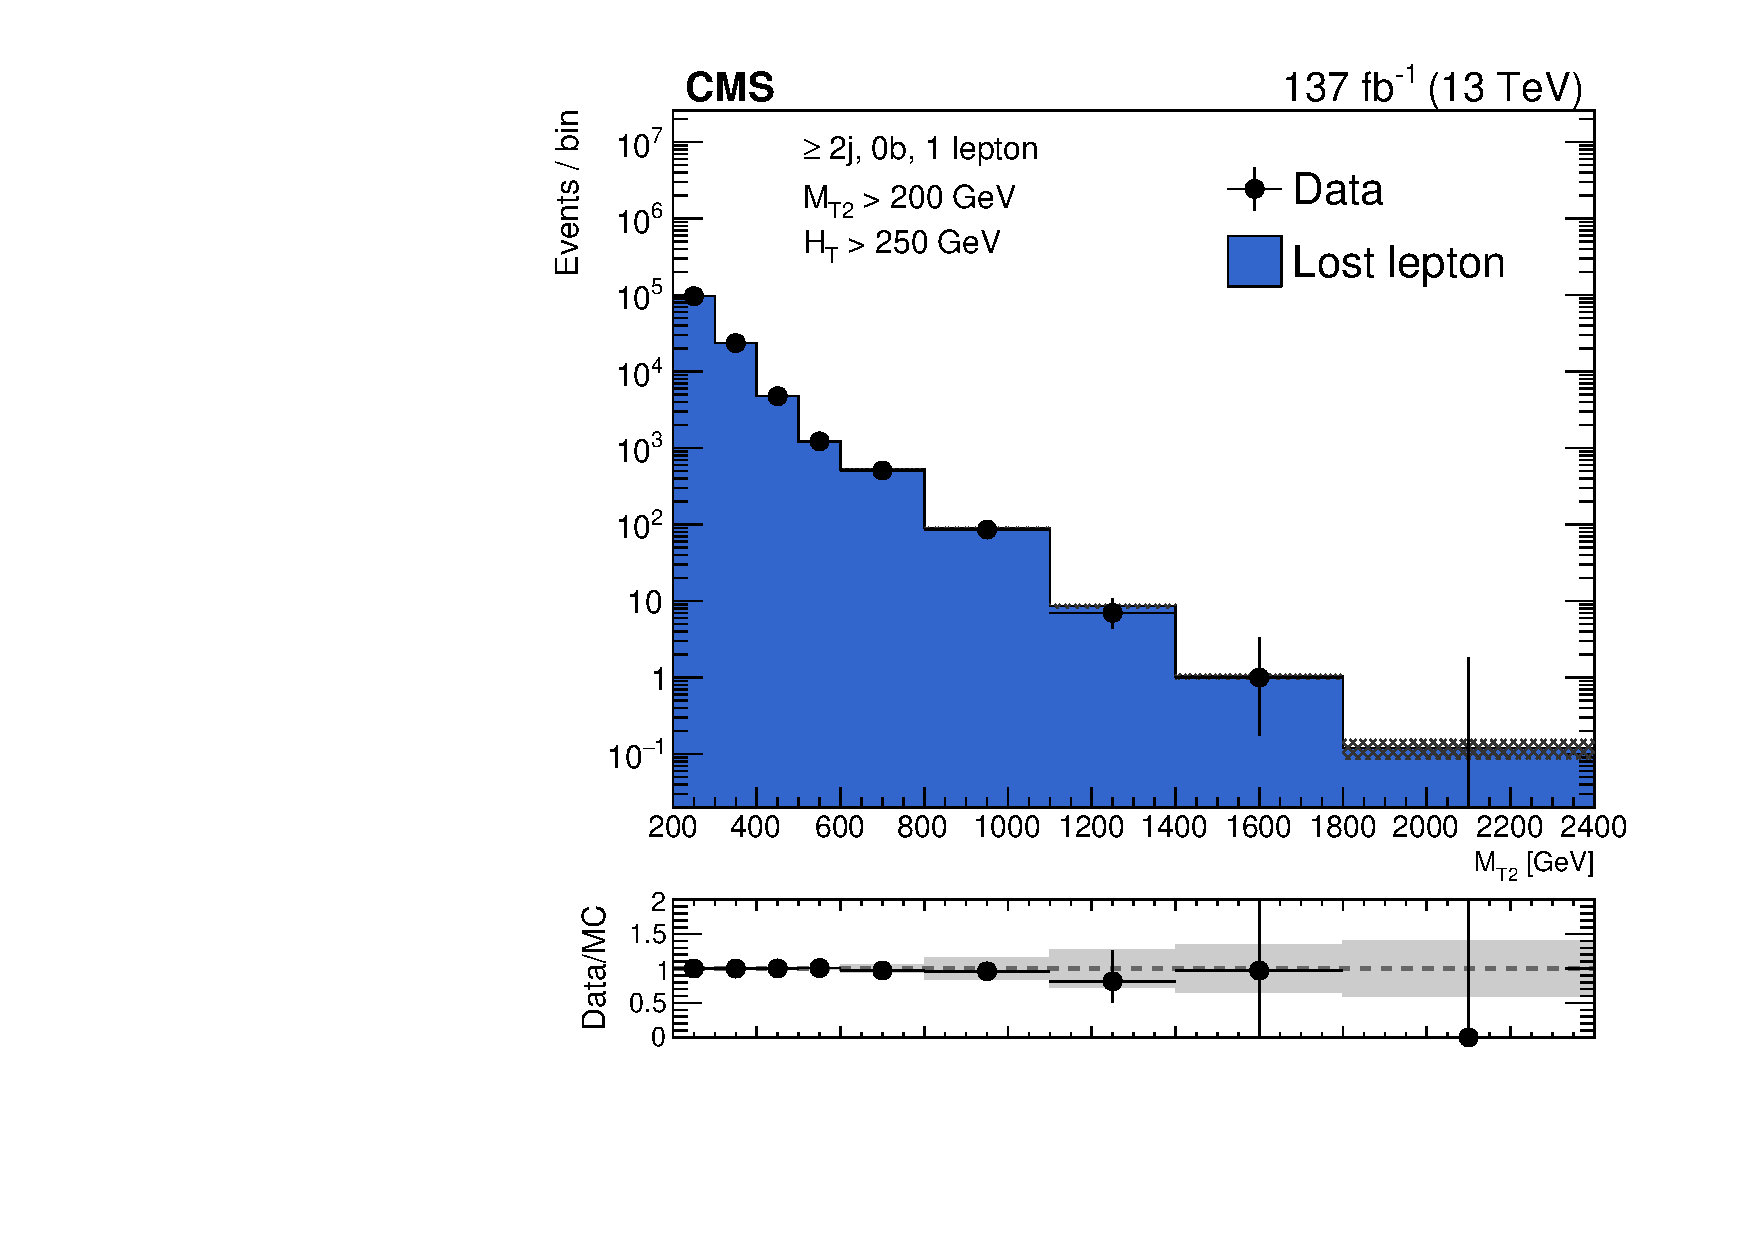
\includegraphics[width=0.48\textwidth]{figures/MT2_2019/Figure_001-a.pdf}
    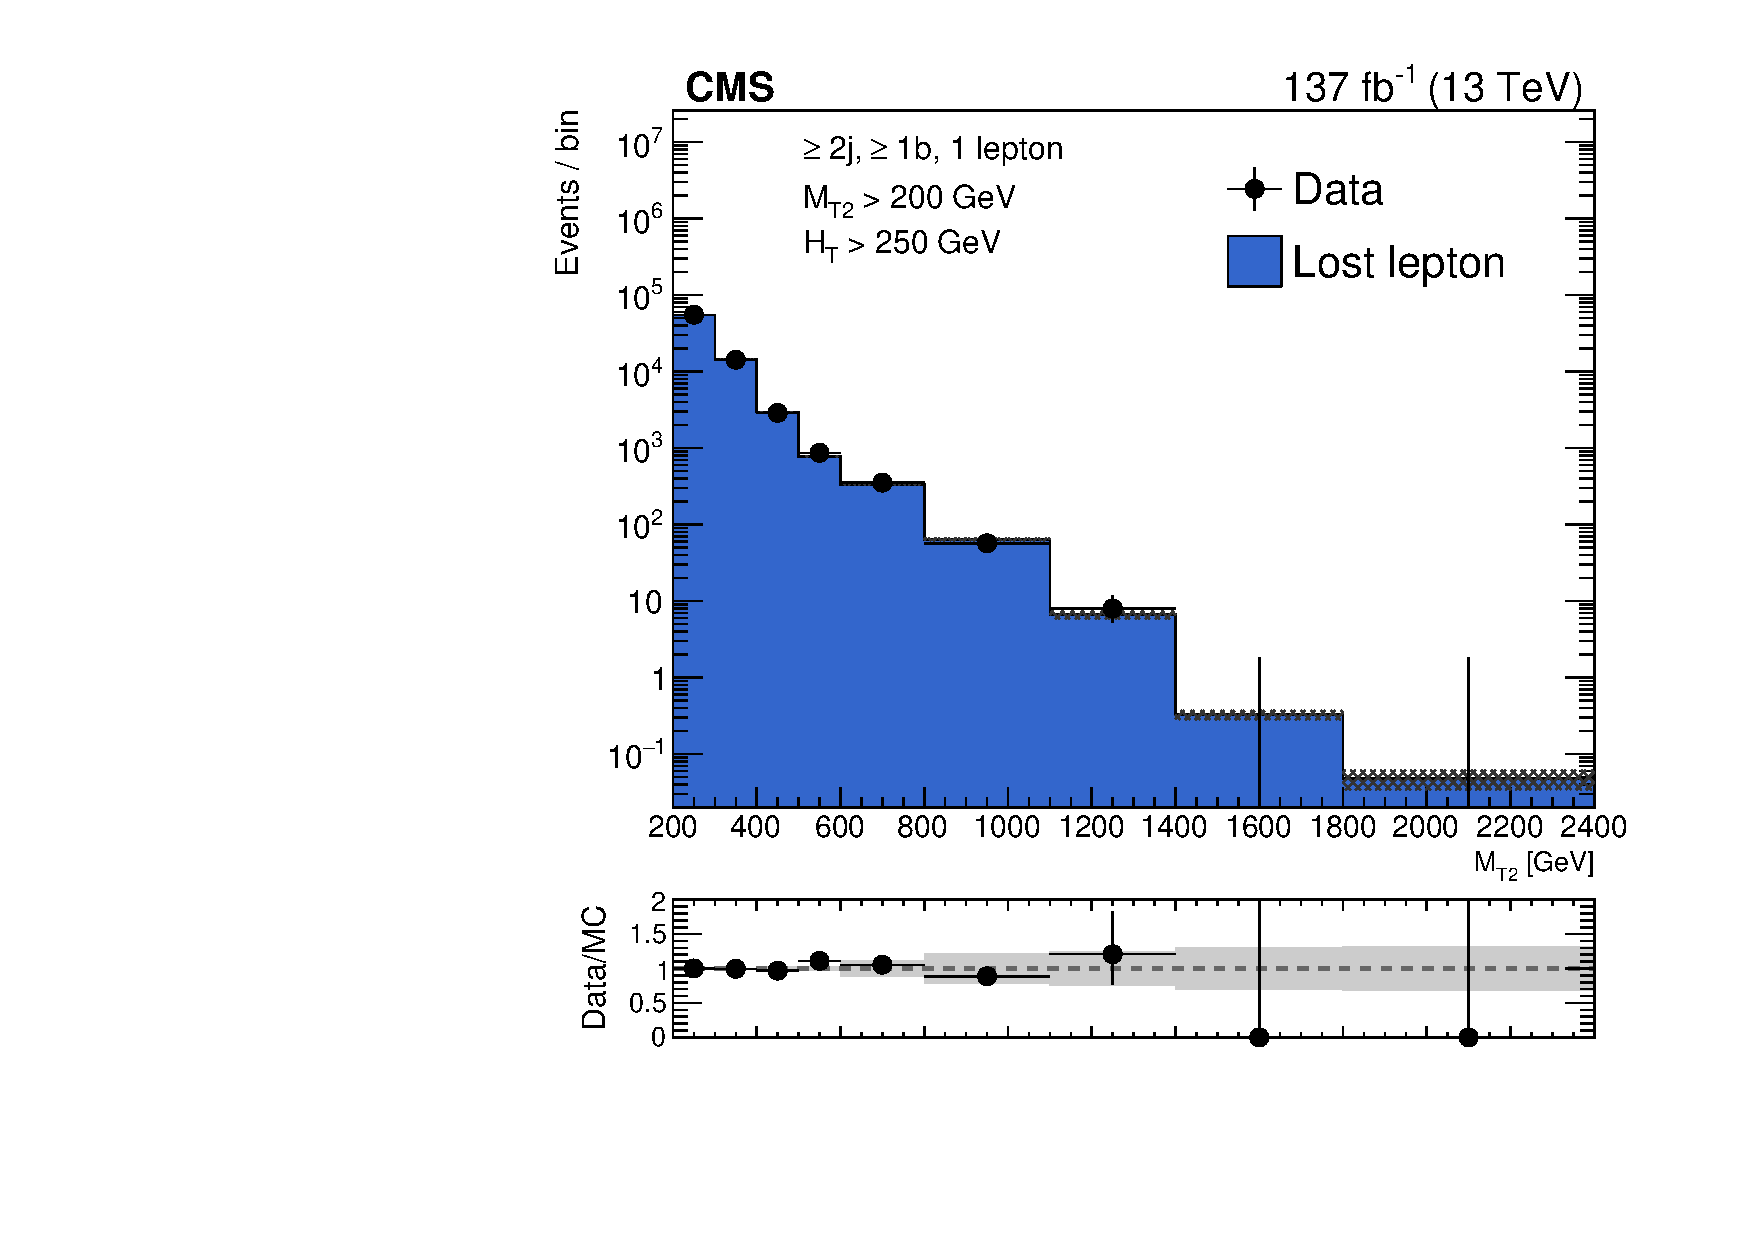
\includegraphics[width=0.48\textwidth]{figures/MT2_2019/Figure_001-b.pdf}
    \caption[Distributions of \mttwo in data and simulation for the single-lepton control region, to check \mttwo modeling in simulation.]
            {Modeling of \mttwo in simulation is checked against data with 0 (left) and 1 b-tagged jets, in events satisfying $\Ht > 250$~GeV, $\met > 250$~GeV if $\Ht < 1200$~GeV and $\met > 30$~GeV otherwise, containing one lepton with $\Mt < 100$~GeV, consistent with a \wlnu decay. 
              The simulation combines all contributing Standard Model processes.
              Even though the simulation is being asked to predict a narrow corner of phase space, and \mttwo is a complex observable depending in detail on all components of the detector, the agreement is remarkable.
              Taken from \cite{MT2_2019}.}
    \label{fig:lepmt2}
  \end{figure}  
